\documentclass[12pt]{scrartcl}
\usepackage[ngerman]{babel}


\usepackage{amsmath, amssymb}

\usepackage{array}  % for the tables

\usepackage{nameref}  % for referencing with name

\usepackage{hyperref}  % for hyperlinks

\usepackage{mathrsfs}

\usepackage{graphicx}  % for the images

\usepackage{xcolor, colortbl}

\usepackage{gensymb} % for \degree

\usepackage{pgfplots}

\usepackage{tabto}

\newcolumntype{P}[1]{>{\centering\arraybackslash}p{#1}}

\usetikzlibrary{arrows}

% \usepgfplotslibrary{external}

% \tikzexternalize

\definecolor{Gray}{gray}{0.85}

\setlength{\parindent}{0cm}

% hyperlinks
\hypersetup{
    colorlinks,
    citecolor=black,
    filecolor=black,
    linkcolor=black,
    urlcolor=black
}

\bibliographystyle{IEEetran}




\author{David Jäggli}

\title{Diskrete Mathematik}



% ---------- Begin Main Document ----------- %



\begin{document}

\maketitle

\tableofcontents

\newpage
\section{Allg}

\subsection{Grundlagen der Logik und Beweise}

\begin{itemize}
    \item Die Regeln der Logik geben mathematischen Aussagen eine präzise Bedeutung.
    \item Konstruktion korrekter mathematischer Argumente
\end{itemize}

\subsection{Aussagen (Propositionen)}
\textbf{Propositionen:}
\begin{itemize}
    \item Bern ist die Bundesstadt
    \item 1 + 1 = 2
    \item Goldbachsche Vermutung: sie ist entweder wahr oder falsch, man weis es noch nicht
\end{itemize}

\textbf{Keine Propositionen:}
\begin{itemize}
    \item Wie spät ist es?
    \item x + 1 = 2
    \item Dieser Satz ist falsch.
\end{itemize}

Begründung: Es handelt sich hier nicht um Aussagen, die entweder wahr oder falsch sind.
Eine Aussage ist wahrheitsdefiniert. In einer Aussage darf nicht offen sein ob die Aussage wahr oder 
falsch sein kann. Sie darf sich auch nicht selbst widersprechen.

% ------------------------------------------------------
\section{Operatoren}

\begin{itemize}
    \item Negotiationsoperator: $\lnot$
    \item Konjunktion $\land$
    \item Disjunktion $\lor$
    \item Implikation $\rightarrow$
    \item Bikonditional $\leftrightarrow$
\end{itemize}



\subsection{Diskunktion}
$p \lor q$\\
Wenn p oder q wahr ist, ist die Aussage wahr (logic OR).


\renewcommand{\arraystretch}{1.5}
\begin{tabular}{ | m{3em} | m{3em} | m{3em} | }
    \hline
    p & q & $p \lor q$\\ 
    \hline
    w & w & w\\ 
    \hline
    w & f & w\\ 
    \hline
    f & w & w\\ 
    \hline
    f & f & f\\ 
    \hline
\end{tabular}


\subsection{Implikation}
$p \rightarrow q$\\
Wenn p dann q


\renewcommand{\arraystretch}{1.5}
\begin{tabular}{ | m{3em} | m{3em} | m{3em} | }
    \hline
    p & q & $p \rightarrow q$\\ 
    \hline
    w & w & w\\ 
    \hline
    w & f & f\\ 
    \hline
    f & w & w\\ 
    \hline
    f & f & w\\ 
    \hline
\end{tabular}


\subsection{Bikonditional}
$p \leftrightarrow q$\\
Wenn beide den gleichen Wahrheitswert haben ist die Aussage wahr.\\
\textbf{Wahrheitstabelle:}\\

\renewcommand{\arraystretch}{1.5}
\begin{tabular}{ | m{3em} | m{3em} | m{3em} | }
    \hline
    p & q & \(p \leftrightarrow q\)\\ 
    \hline
    w & w & w\\ 
    \hline
    w & f & f\\ 
    \hline
    f & w & f\\ 
    \hline
    f & f & w\\ 
    \hline
\end{tabular}

\subsection{Prioritäten}
\renewcommand{\arraystretch}{1.5}
\begin{tabular}{ | m{4em} | m{4em} | }
    \hline
    Operator & Priorität\\ 
    \hline
    $\lnot$ & 1\\ 
    \hline
    $\land$ & 2\\ 
    \hline
    $\lor$ & 2\\ 
    \hline
    $\rightarrow$ & 3\\ 
    \hline
    $\leftrightarrow$ & 3\\ 
    \hline
\end{tabular}


\section{Aussagen}

\subsection{Tautologie und Wiederspruch}
Tautologie ist eine Aussage, welche immer wahr ist.\\
Ein Wiederspruch ist eine Aussage, welche immer falsch ist.

\subsection{Logische Äquivalenzen}
Die Aussage p und q heissen logisch äquivalent, falls \(p \leftrightarrow q\) eine Tautologie ist. 
Man schreibt dann \(p \Leftrightarrow q\) oder
\(p \equiv q\) bzw. $p \sim q$

\subsection{Logische Äquivalenzregeln}
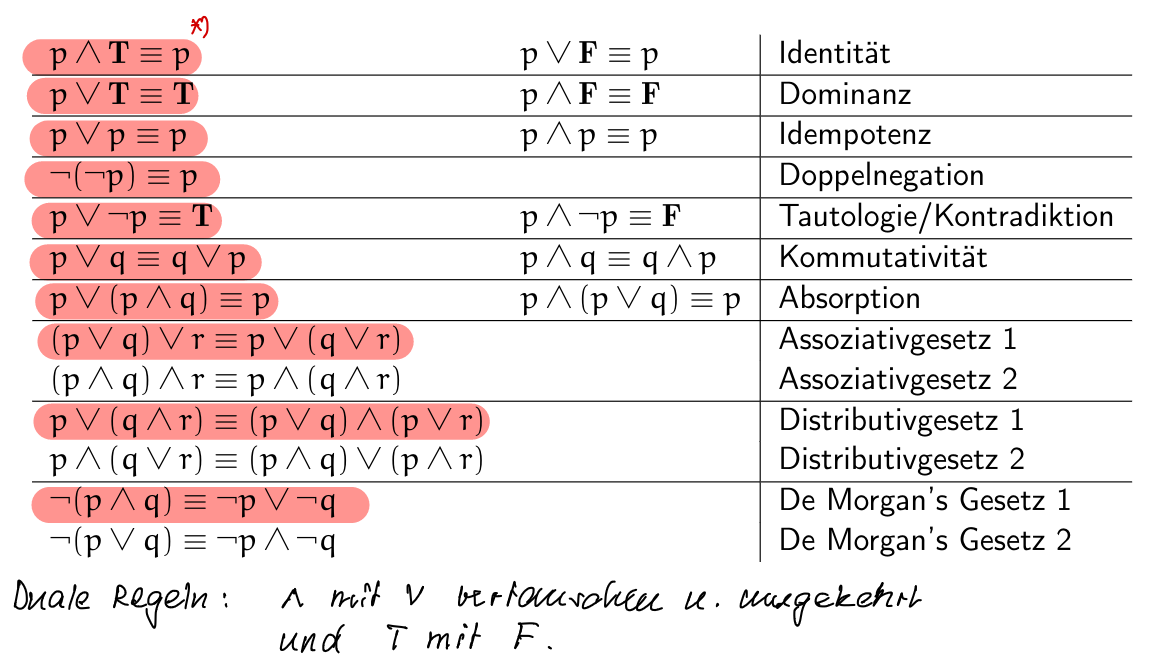
\includegraphics[width=14cm]{img/logic_equivalence_rules.png}

Weiterführend:\\
$p \rightarrow q \equiv \lnot p \lor q$


\newpage
\textbf{Beispiel angewandte logische Äquivalenzregeln}\\
Beispiel 1:\\
$\left(p \lor \lnot(q \land p)\right) \land \left(r \lor (s \lor r)\right)$\\
$\equiv (p \lor \lnot q \lor \lnot p) \land (r \lor r \lor s)$\\
$\equiv (T \lor \lnot q) \land (r \lor s)$\\
$\equiv T \land (r \lor s)$\\
$\equiv r \lor s$
 \\
 \\
 \\

Beispiel 2:\\
$(a \rightarrow (b \rightarrow c)) \rightarrow ((a \rightarrow b)\rightarrow (a \rightarrow c))$\\
$\equiv (a \rightarrow (\lnot b \lor c)) \rightarrow ((\lnot a \lor b) \rightarrow (\lnot a \lor c))$\\
$\equiv (\lnot a \lor (\lnot b \lor c)) \rightarrow (\lnot(\lnot a \lor b) \lor (\lnot a \lor c))$\\
$\equiv (\lnot a \lor \lnot b \lor c) \rightarrow ((a \land \lnot b) \lor \lnot a \lor c)$\\
$\equiv (\lnot a \lor \lnot b \lor c) \rightarrow ((a \lor \lnot a) \land (\lnot b \lor \lnot a) \lor c)$\\
$\equiv (\lnot a \lor \lnot b \lor c) \rightarrow (\lnot b \lor \lnot a \lor c)$\\
$\equiv$ X $\rightarrow$ X\\
$\equiv \lnot$X $\lor$ X\\
$\equiv$ T\\

\section{Quantoren}
Wird ein Quantor auf die Variable x angewandt, dann nennt man diese Variable \textit{gebunden}, ansonsten \textit{frei}.
\subsection{Prädikate}
Ein Prädikat ist ein Wortkonstrukt, welches mindestens eine Variable enthält.\\
$P(x) =$ ''$x > 3$''\\
Die Aussage $P(4) = 4 > 3$ ist wahr, während $P(2) = 2 > 3$ falsch ist.

\subsection{Allquantor}
Ist $P(x)$ wahr für alle x aus einer bestimmten Universalmenge, dann schreibt man $\forall x P(x)$.
Gelesen wird dies, "für alle $x$ gilt $P(x)$".\\
Falls es nur auf eine Bestimmte Zahlenmenge zutrifft (z.B. $\mathbb{Z}$) dann schreibt man:\\
$\forall x \in \mathbb{Z}$ ist wahr.

\subsection{Existenzquantor}
Ist $P(x)$ wahr für mindestens ein $x$ aus einer bestimmten Universalmenge, dann schreibt man $\exists x P(x)$
und liest: "es existiert ein $x$ für welches $P(x)$ wahr ist".


\subsection{Verschachtelte Quantoren}
Die Reihenfolge der Quantoren ist wesentlich; ausser alle Quantoren sind vom gleichen Typ (also Allquantoren oder Existenzquantoren)!


\newpage
\section{Beweise}
\begin{itemize}
    \item Ein Satz (Theorem) ist eine Aussage, von der man zeigen kann, dass sie wahr ist.
    \item Um zu zeigen, dass ein Satz wahr ist, verwendet man eine Abfolge (Sequenz) von Aussagen, die zusammen ein Argument, genannt Beweis ergeben.
    \item Aussagen können Axiome oder Postulate enthalten (grundlegende Annahmen der mathematischen Strukturen).
    \item Durch logisches (also gewissen Regeln gehorchendes) schliessen werden Folgerungen gemacht, die zusammen den Beweis ergeben.
    \item Ein Lemma ist ein einfacher Satz, der in Beweisen von komplizierteren Sätzen verwendet wird.
    \item Ein Korollar ist eine einfache Folgerung eines Satzes.
\end{itemize}


% ----------- Mengen ----------- %

\newpage
\section{Mengen}

Eine Menge ist eine ungeordnete Zusammenfassung wohldefinierter, unterscheidbarer
Objekte, genannt \textit{Elemente}, zu einem Ganzen. Für irgendein Objekt $x$ 
gilt dann bezüglich der Menge $A$ entweder $x \in A$ oder dann $x \notin A$.

\textbf{Beispiel:}\\
Endliche Mengen lassen sich durch Aufschreiben der in ihnen enthaltenen Elemente beschreiben.
z.B. die Menge aller natürlichen Zahlen kleiner als 101:\\
$A = {0, 1, 2, ..., 99, 100}$ (aufzählend notiert)\\
$99 \in A$ aber $101 \notin A$ (beschreibend notiert)\\

andere Schreibweisen sind: \\

$A = {n \in \mathbb{N} | n < 101} = {n \in \mathbb{N} : n <= 100} = {n|n \in \mathbb{N} \land n <= 100}$\\

\subsection{Gleichheit, elementare Mengen}
Zwei Mengen $A$ und $B$ sind \textbf{gleich} ($A = B$), falls sie dieselben Elemente enthalten.
$(A \subset B) \land (B \subset A)$\\

\textbf{Einige bekannte Mengen:}\\
$\mathbb{N}$ - \quad Menge der natürlichen Zahlen $(\mathbb{N}^* = \mathbb{N} \setminus \{0\})$\\
$\mathbb{Z}$ - \quad Menge der ganzen Zahlen\\
$\mathbb{Z}^+$ - \quad Menge der positiven ganzen Zahlen\\
$\mathbb{Q}$ - \quad Menge der Brüche\\
$\mathbb{R}$ - \quad Menge der reellen Zahlen\\
$\mathbb{C}$ - \quad Menge der komplexen Zahlen\\

\subsection{Spezielle Mengen}
\textbf{Teilmenge:} $A$ ist Teilmenge von $B$, geschrieben $A \subset B$, genau dann, wenn
$\forall x (x \in A \rightarrow x \in B)$: es gilt $A \subset A$!\\

\textbf{Leere Menge:} Für jede Menge $A$ gilt: $\emptyset \subset A$.\\

\textbf{Kardinalität:} Ist $S$ eine endliche Menge, dann bezeichnet $|S|$ die Kardinalität. Die
Kardinalität ist die Anzahl Elemente von $S$.\\

\textbf{Potenzmenge}: Die Potenzmenge $P(S)$ oder $2^S$ der Menge $S$ besteht aus der Menge aller
Teilmengen $A \subset S$.\\

\textbf{Beispiel:}\\
Bestimmen Sie die Potenzmenge von $S= \{1,2\}$\\
$S = \{1,2\}$\\
\quad $P(S) = 2^S = \{\emptyset, \{1\}, \{2\}, \{1, 2\}\}$\\
Es gilt allgemein $|2^S| = 2^{|S|}$


\subsection{Das Kreuzprodukt zweier Mengen / kartesisches Produkt}
$ A \times B = \{(a, b)|a \in A \land b \in B\}$\\
Reihenfolge ist entscheidend, $A \times B \neq B \times A$\\
$|A \times B| = |A| \cdot |B|$\\

\textbf{Beispiel:}
$A \times B = \{(1,a), (2,a), (3,a), (1,b), (2,b), (3, b)\}$


\subsection{Mengenoperationen}
\subsubsection{Komplement}
Ist $A$ eine Teilmenge der Menge $M$, so bezeichnet\\

$A^c = \overline{A} =  \{m \in M | m \notin A\}$\\

das Komplement von $A$ bezüglich $M$.

\subsubsection{Durchschnitt}
Sind $A$ und $B$ Teilmengen einer Menge $M$, so bezeichnet\\

$A \cap B = \{m \in M | m \in A \land m \in B\}$\\

den  Durchschnitt von $A$ und $B$.


\subsubsection{Vereinigung}
Sind $A$ und $B$ Teilmengen einer Menge $M$, so bezeichnet\\

$A \cup B = \{m \in M | m \in A \lor m \in B\}$\\

die Vereinigung von $A$ und $B$.


\newpage
\subsubsection{Differenz}
Sind $A$ und $B$ Teilmengen einer Menge $M$, so bezeichnet \\

$B \setminus A = \{m \in M | m \in B \land m \notin A\}$\\

die Differenz


\subsection{Set Operatoren}
\renewcommand{\arraystretch}{1.5}
\begin{tabular}{ | m{7em} | m{7em} | }
    \hline
    Allg. Operator & Set Operator \\ 
    \hline
    $p \lor q$ & $A \cup B$ \\ 
    \hline
    $p \land q$ & $A \cap B$ \\ 
    \hline
    $\lnot p$ & $\overline{A} $ \\ 
    \hline
\end{tabular}

\subsubsection{Rechenregeln}
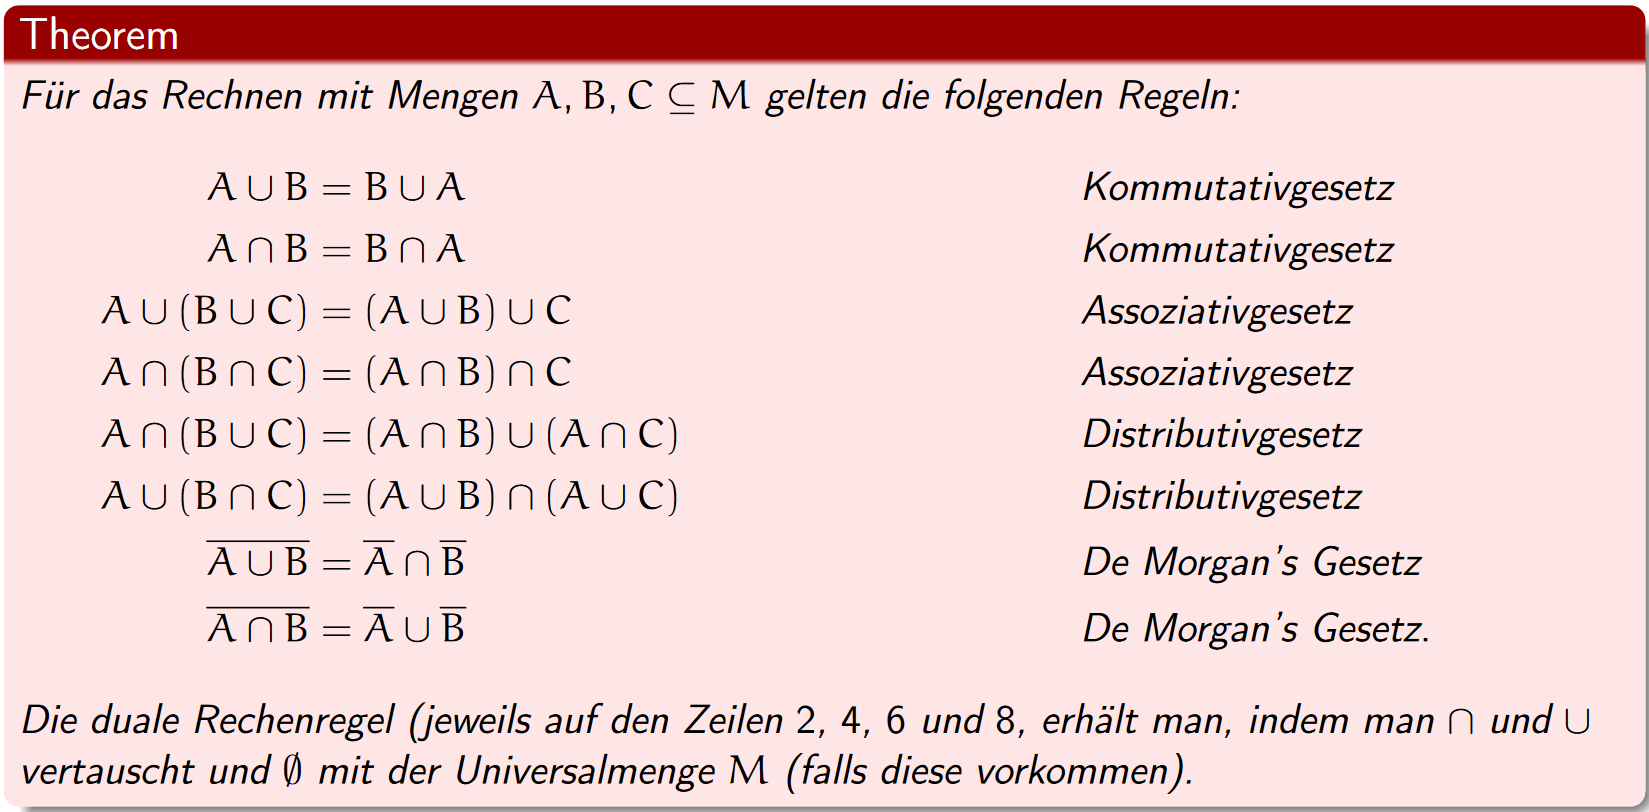
\includegraphics[width=15cm]{img/Rechenregeln_mit_mengen.png}

\subsubsection{Mengen Identitäten}
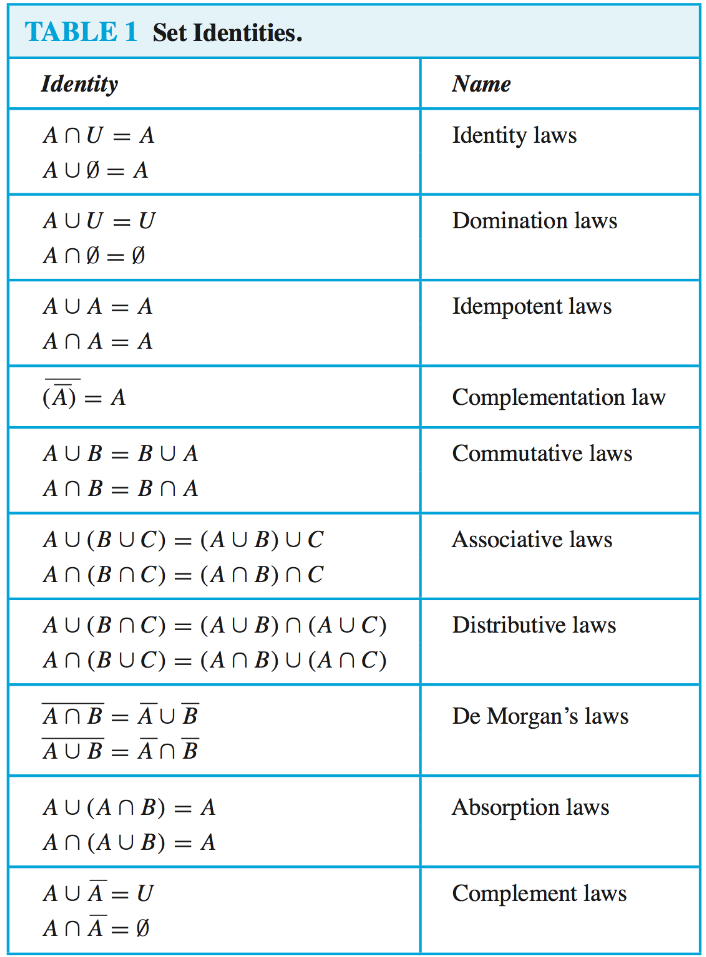
\includegraphics[width=15cm]{img/set_identities.png }




\section{Funktionen}
\subsection{Injektive Funktionen}
Eine Funktion heisst injektiv, wenn jedes $x$ auf eine eigenes $y$ zeigt.

\subsection{Surjektive Funktionen}
Eine Funktion heisst surjektiv, falls für jedes Element $y$ ein Element $x$ existiert, so dass $f(x) = y$ gilt.

\subsection{Bijektive Funktionen}
Eine Funktion heisst bijektiv, falls sie injektiv und surjektiv ist. Das bedeutet, dass jedes Element $y$ genau
ein zugehöriges Element $x$ hat.\\

Bijektive Funktionen sind umkehrbar. Man muss einfach die Pfeile umkehren und damit entsteht
aus $f$ die Umkehrfunktion $f^{-1}$.


\subsection{Zusammengesetzte Funktionen}
Gegeben seien zwei Funktionen, so dass der Wertebereich von $g$ im Definitionsbereich von $f$ enthalten ist.
Dann kann man die so genannte \textbf{zusammengesetzte Funktion} oder \textbf{Komposition} von $f$
und $g$ bilden:\\
$F = f \circ g$ : $X \longmapsto Y$, $x \longmapsto f(g(x))$

\subsection{Umkehrfunktionen}
Wenn man die Umkehrfunktion auf das Ergebnis der Ursprungsfunktion mit einem $x$-Wert anwendet
erhält man wieder $x$. Heisst:\\
$f^{-1}(f(x)) = x$


\newpage
\section{Folgen}
\subsection{Definition}
Eine \textbf{Folge} ist eine Abbildung von $\mathbb{N}$ (oder auch $\mathbb{N}^* = \mathbb{N} \setminus \{0\}$) in eine Menga $A$:\\
$\{\cdot\}$:$\mathbb{N} \mapsto A$, $n \mapsto a_n$\\
Man nennt $a_n$ das Glied der Folge mit der Nummer $n$. Die Folge wird auch mit \{$a_n$\} oder ($a_n$) bezeichnet.\\

\textbf{Example:}\\
Man schreibe die ersten sechs Glieder der Folge auf, deren k. Glied gegeben ist durch $a_k = \frac{1}{k}$. \\

$a_k = \left(1,  \dfrac{1}{2}, \dfrac{1}{3}, \dfrac{1}{4}, \dfrac{1}{5}\dots\right)$


\subsection{Die geometrische Folge}
Bei einer geometrischen Folge ist der Quotient zweier aufeinander folgender Glieder immer
gleich, nämlich q. Das bedeutet, dass $\frac{a_{k+1}}{a_k}$ immer gleich ist.


\subsection{Summen}
Dank Summenzeichen lassen sich Summen einfacher schreiben:
\[\sum_{j=m}^{n} a_j = a_m + a_{m+1} + a_{m+2} + \dots + a_n\]

\[\sum_{j=m}^{n} a_j = \sum_{i=0}^{n-m} a_{m+i} = \sum_{k=1}^{n-m+1} a_{m+k-1}\]


Addiert man die Glieder einer arithmetischen Folge ($a_k$), entsteht die \textbf{arithmetische Reihe:}

\[\sum_{k=0}^{n-1} a_k = n \frac{a_0 + a_{n-1}}{2}\]


\newpage
\textbf{Nützliche Summenformeln:}

\renewcommand{\arraystretch}{2.5}
\begin{center}
    \begin{tabular}{  m{10em} | P{10em} }
        \hline
        Summe & geschlossene Form \\
        \hline
        $\sum_{k=0}^{n} x^k$                        & $\frac{x^{n + 1} - 1}{x - 1}$               \\ 
        $\sum_{k=0}^{n} 2^k$                        & $2^{k + 1} - 1$               \\ 
        $\sum_{k=1}^{n} k$                          & $\dfrac{n(n + 1)}{2}$         \\ 
        $\sum_{k=1}^{n} k^2$                        & $\dfrac{n(n + 1)(2n + 1)}{6}$ \\ 
        $\sum_{k=1}^{n} k^3$                        & $\dfrac{n^2(n + 1)^2}{4}$     \\ 
        $\sum_{k=0}^{\infty} x^k$, $|x| < 1$        & $\dfrac{1}{1 - x}$            \\ 
        $\sum_{k=1}^{\infty} kx^{k-1}$, $|x| < 1$   & $\dfrac{1}{(1-x)^2}$          \\ 
        \hline
    \end{tabular}
\end{center}


\subsection{Produkte}
Dank dem Produktzeichen lassen sich Produkte einfacher schreiben:\\


\[a_m \cdot a_{m+1} \cdot a_{m+2} \dots a_n = \prod_{j=m}^{n} a_j \quad\quad n \geqslant m\]

Die Fakultät lässt sich mithilfe des Produktzeichens wie folgt schreiben:\\
\[n! = 
\begin{cases}
    1 & n=0 \\
    n(n - 1)(n - 2) \dots 2 \cdot 1 = \prod_{k=1}^{n}k & n > 0
\end{cases}\]


Nützliche Abkürzung:
\[\prod_{i=1}^{n} i = \frac{n \cdot (n + 1)}{2}\]

\newpage
\section{Wachstum von Funktionen / Big-O}

\subsection{Definition}
Seien $f$ und $g$ Funktion von $\mathbb{Z}$ oder ($\mathbb{R}$). Dann sagt man "$f(x)$ ist $\mathcal{O}(g(x))$", falls es
Konstanten $C$ und $k$ gibt, so dass gilt:

$|f(x)| \leq C|g(x)|$, $\forall x > k$ Lies: "f(x) ist gross-O von g(x), man schreibt: $f(x) \in \mathcal{O}(g(x))$.

\begin{itemize}
    \item Meist ist f eine komplizierte Funktion, wie z.B. $f(x) = (x^2 + 1) ln x + (2^x + x^4)$
    \item Man möchte für g eine möglichst einfache, nicht zu schnell wachsende Funktion, wie z.B. $x$, $x^2$ \dots
    \item Ziel ist es herauszufinden, wie sich f(x) für sehr, sehr grosse $x$ verhält, und zwar verglichen mit der einfacheren Funktion $g$.
    \item k ist der kleinste Wert von $x$, für den die obige Ungleichung noch gilt!
\end{itemize}

Also wir wollen für sehr grosse $x$, eine einfachere Funktion zu finden.


\subsection{Example}
Für $f(x) = x^2 + 2x + 1$ ist $\mathcal{O}(x^2)$.\\
Das heisst bei sehr grossen $x$ entspricht die Funktion $f(x) =  x^2$

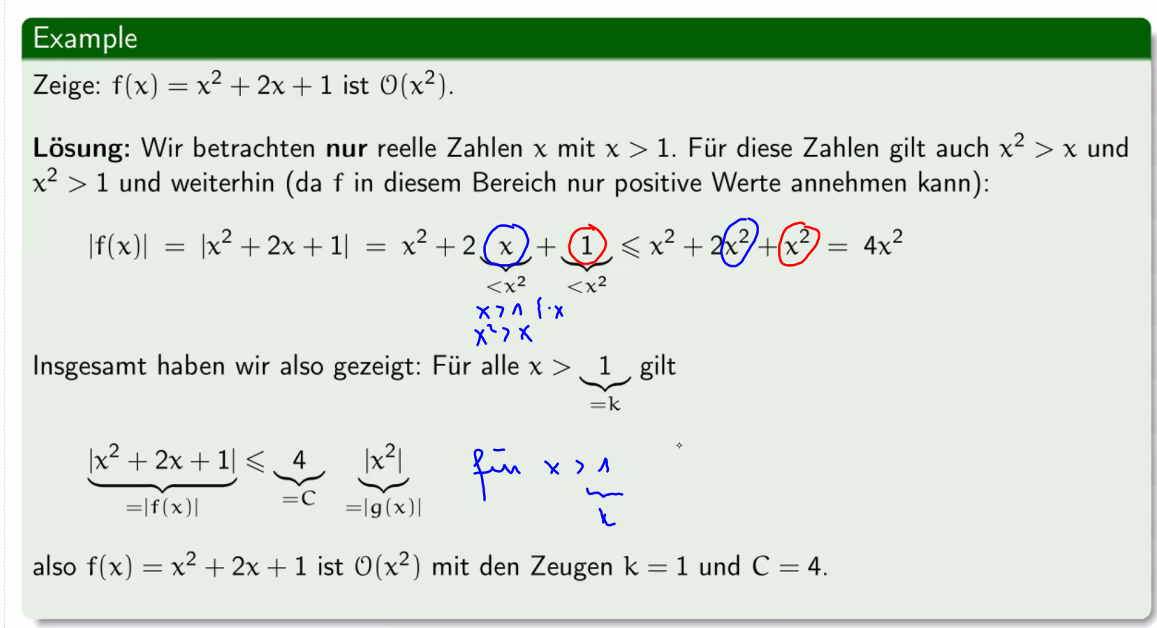
\includegraphics[width=15cm]{img/wachstum_example_1.png}
\newpage
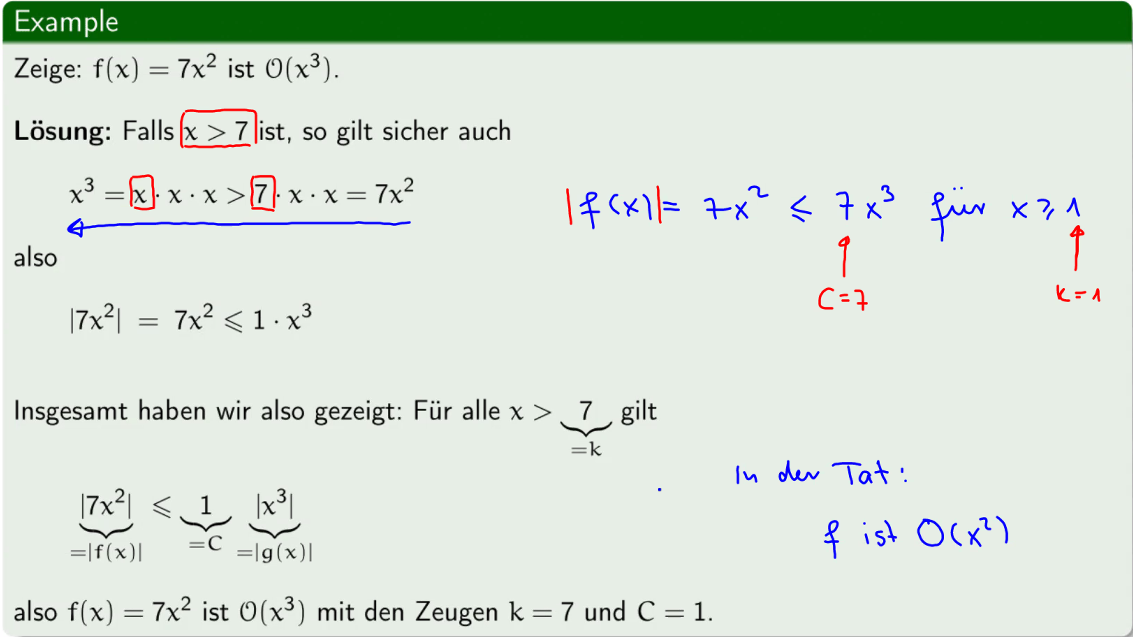
\includegraphics[width=15cm]{img/wachstum_example_2.png}


\subsection{Polynome}
Für das Polynom $\sum_{k=0}^n a_k x^k$ gilt $f(x)$ ist $\mathcal{O}(x^n)$. Das heisst
die höchste Potenz von x gibt den Ton an.\\

\textbf{Beispiel:}\\
Es gilt immer: $|a + b| \leq |a| + |b|$\\

$f(x) = 5x^6 - 3x^2 + x - 10$\\
$|f(x)| \leqslant 5x^6 + 3x^2 + x + 10$\\
$|f(x)| \leqslant 5x^6 + 3x^6 + x^6 + 10x^6$\\
$|f(x)| \leqslant 5x^6 + 3x^6 + x^6 + 10x^6$ für $x \geqslant 1$\\
$|f(x)| = 19x^6$\\

also $f$ ist $\mathcal{O}(x^6)$ mit Zeugen $k=1$ und $C = 19$


\newpage
\section{Zahlen und Division}
\subsection{Definition}
Falls $a$ ein Teiler von $b$ ist schreibt man $a \mid b$ und sagt ``a teilt b'' oder ``a ist ein Teiler von b''.

\subsection{Modulare Arithmetik}
Sei $m \in \mathbb{N} \backslash \{0\}$, dann nennt man zwei ganze Zahlen a und b kongruent modulo m, falls $m\mid (a - b)$.
Das heisst a und b liegen ein Vielfaches von m auseinander. Man schreibt dann $a \equiv b$ mod $m$ und sagt:
``a ist kongruent zu b modulo m''.\\

$13 \equiv 1$ mod 4 denn $4 \mid (13 - 1)$\\
$13 \equiv 1$ mod 3 denn $3 \mid (13 - 1)$\\
$13 \not\equiv  1$ mod 5 denn $5 \nmid (13 - 1)$\\

Die Schreibweise bedeutet $13 - 1$ (12) ist ein Vielfaches von 4.\\

\subsection{Der Euklidische Algorithmus}
Effiziente Methode um ggT zu finden.

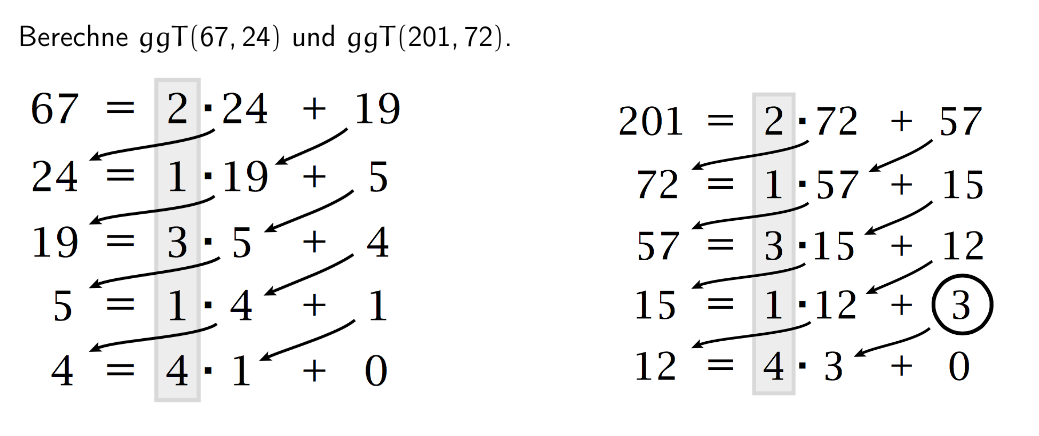
\includegraphics[width=15cm]{img/euqlidic_algorithm.png}

ggT ist jeweils 1 und 3.


\newpage
\subsection{Erweiterter euklidischer Algorithmus}
Lösung der Gleichung mit der diophantischen Gleichung.\\

Finde $x$,$y \in \mathbb{Z}$ mit $211 \cdot x + 13 \cdot y = 1$\\ 

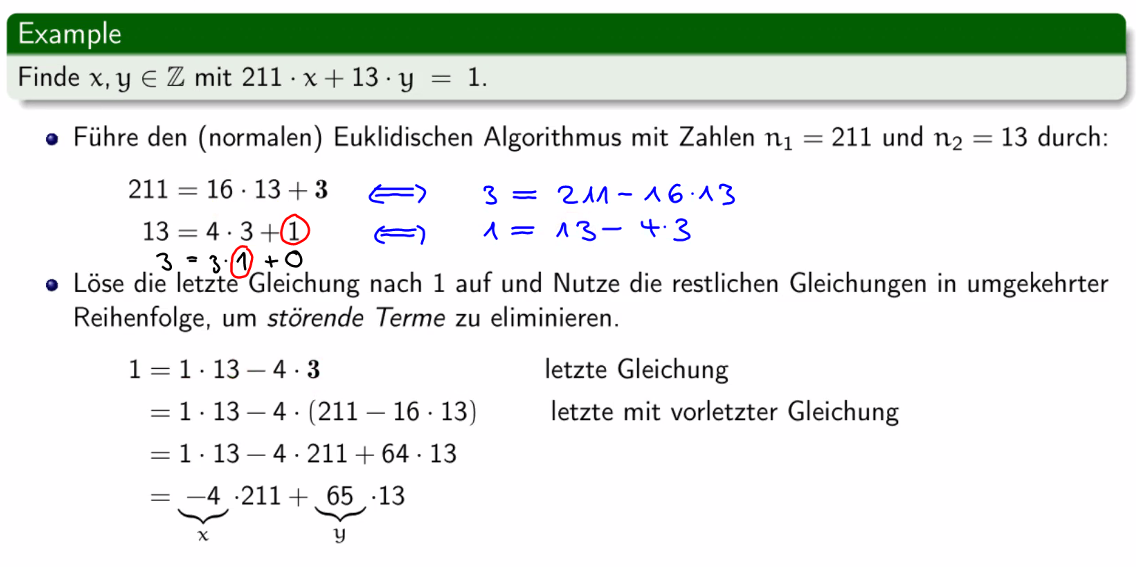
\includegraphics[width=14cm]{img/erweiterter_euklidischer_algorithmus.png}

Mit einem nächsten Beispiel: zuerst (blau) der normale euklidische Algorithmus machen
und danach der erweiterte machen (rot) von unten nach oben. Dann hat man am Schluss
x und y in der Gleichung.

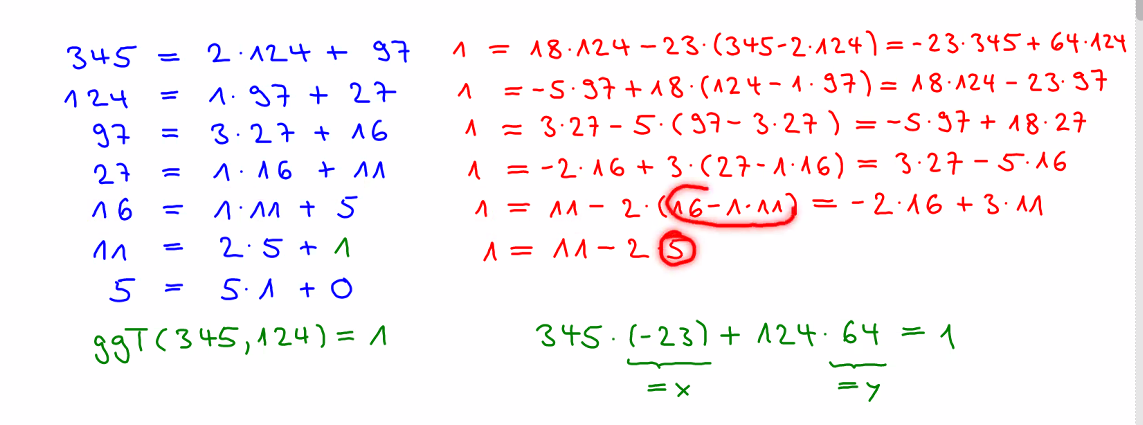
\includegraphics[width=14cm]{img/erweiterter_euklidischer_algorithmus_beispiel2.png}

\newpage
\section{Matrizen}
\subsection{Definition}
Eine m $\times$ n-Matrix ist eine rechteckige Anordnung von Zahlen in m Zeilen und n
Spalten.\\

\renewcommand{\arraystretch}{1}
\textbf{A} = 
$
\begin{bmatrix}
    a_{1,1} & a_{1,2} & \cdots & a_{1,n}\\
    a_{2,1} & a_{2,2} & \cdots & a_{2,n}\\
    \vdots & \vdots & \ddots & \vdots\\
    a_{m,1} & a_{m,2} & \cdots & a_{m,n}
\end{bmatrix}$\\


Kurzschreibform: \textbf{A} = [$a_{i,j}$]\\


\subsection{Addition von Matrizen}

Addition von Matrizen erfolgt jeweils durch die Addition der einzelnen Positionen


\subsection{Multiplikation mit einer Zahl}
Einfach jede Zahl multiplizieren.


\subsection{Matrixmultiplikation}
\textbf{C = AB}, wobei die Anzahl Spalten in \textbf{A} gleich der Anzahl Reihen in \textbf{B}
sein muss

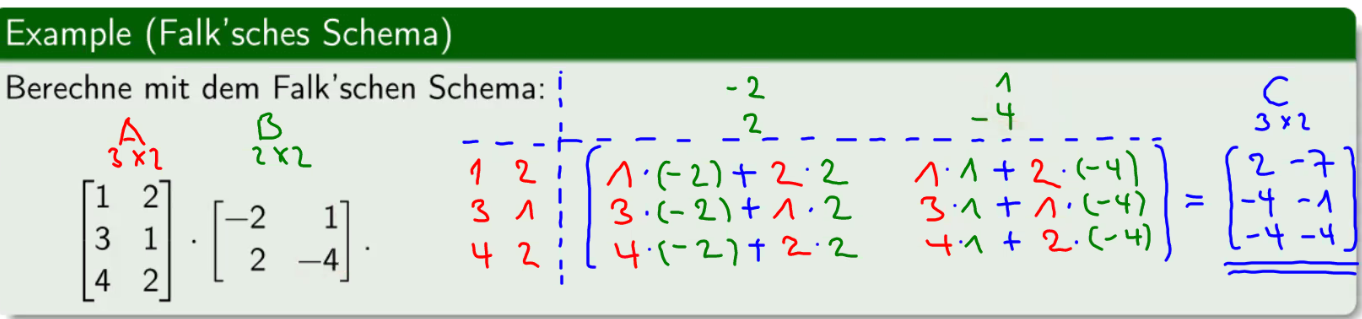
\includegraphics[width=15cm]{img/matrizenmultiplikation.png}


\subsection{Einheitsmatrix}
Eine Einheitsmatrix $\mathbf{I_n}$ ist eine Matrix bei der alle Elemente auf
der Diagonalen Eins und alle anderen Null sind.\\


\subsection{Inverse Matrix}
Das Inverse ($\mathbf{-A}$) ist eine Matrix mit jedem Wert negiert.\\


\newpage
\subsection{Transporierte Matrix}
Eine transponierte Matrix ist eine, bei der die Spalten und Reihen vertauscht wurden.\\

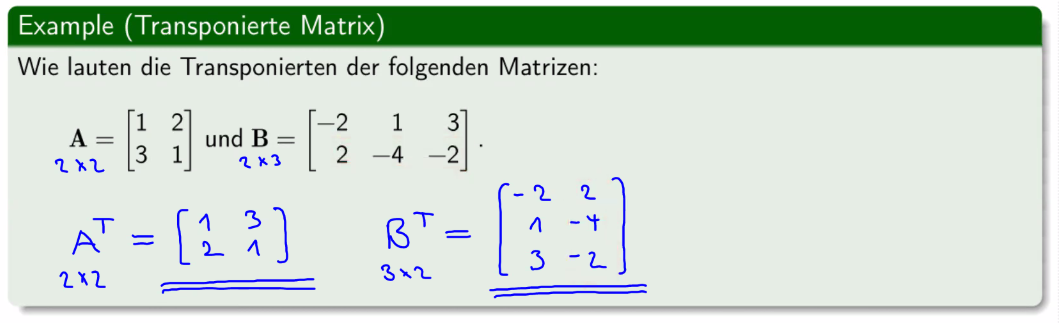
\includegraphics[width=15cm]{img/transponierte_matrix.png}

\subsection{Matrizen Eigenschaften}
Keywords: symmetrisch, antisymmetrisch, Einheitsmatrix, k-te Potenz

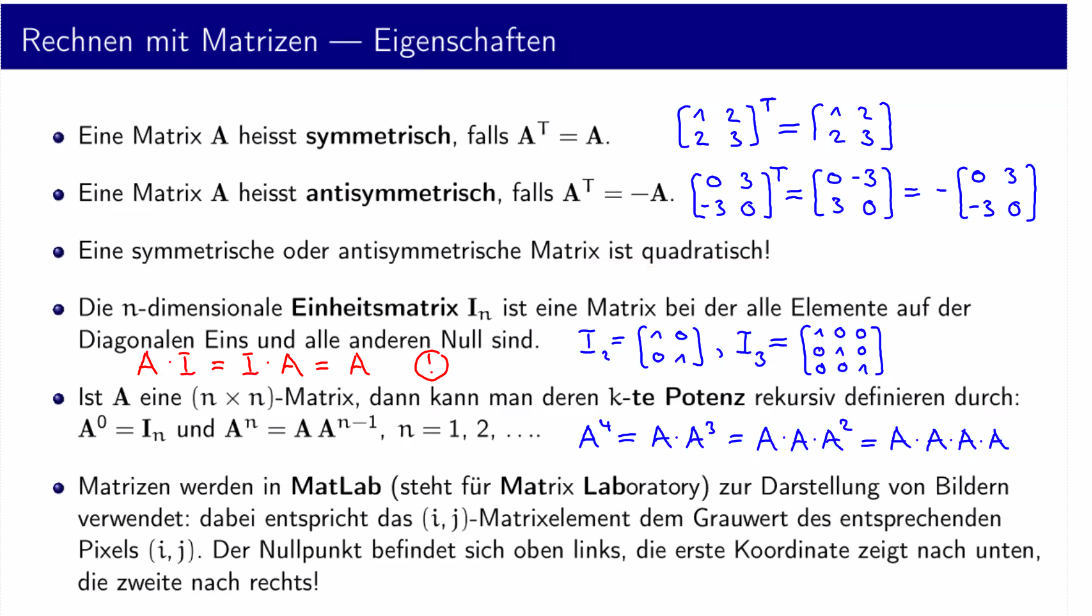
\includegraphics[width=16cm]{img/matrizen_eigenschaften.png}


\newpage
\subsection{Matrizen Rechenregeln}
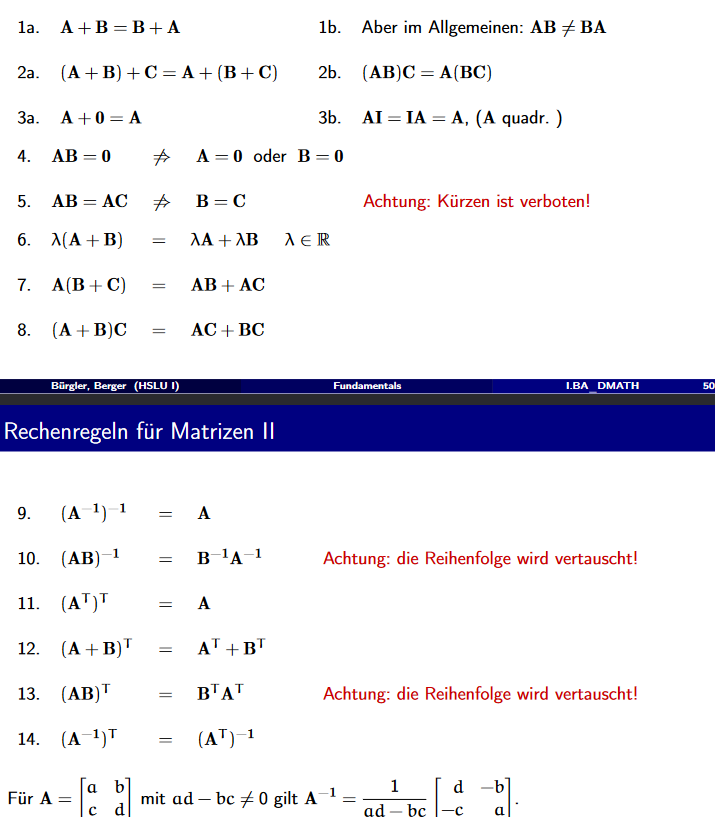
\includegraphics[width=14cm]{img/matrizen_rechenregeln.png}


\newpage
\subsection{Determinante}
\subsubsection{2x2 Matrix}
Die Determinante der Matrix \textbf{A} $= \begin{bmatrix}
    A_{1,1} & A_{1,2}\\
    A_{2,1} & A_{2,2}
\end{bmatrix}$
ist $|A|$ = $det(\textbf{A}) = A_{1,1} \cdot A_{2,2} - A_{1,2} \cdot A_{2,1}$\\

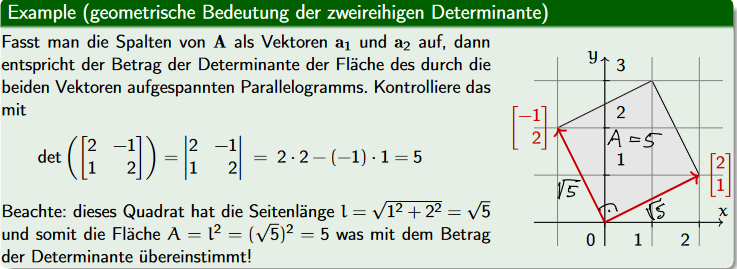
\includegraphics[width=14cm]{img/determinante.png}

\subsubsection{3x3 Matrix}
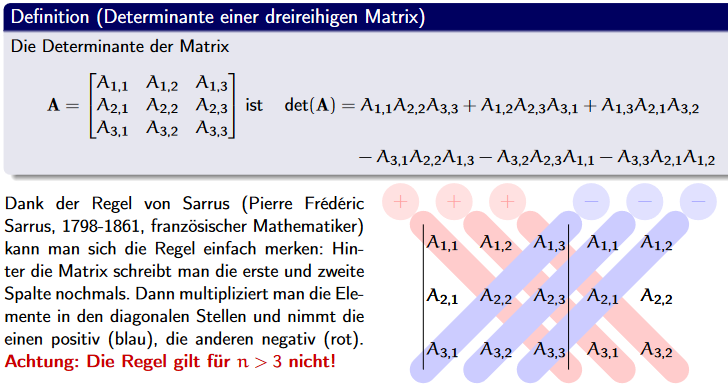
\includegraphics[width=14cm]{img/determinante_2.png}


\subsection{Admittanzmatrix, Adjazenzmatrix, Gradmatrix}

Siehe Ende Graphentheorie.

\newpage
\subsection{Null-Eins Matrizen}
Auch boolesche Matrizen genannt.\\

Boolesches Matrizen Produkt wird folgendermassen geschrieben: $\mathbf{A} \odot  \mathbf{B}$.\\

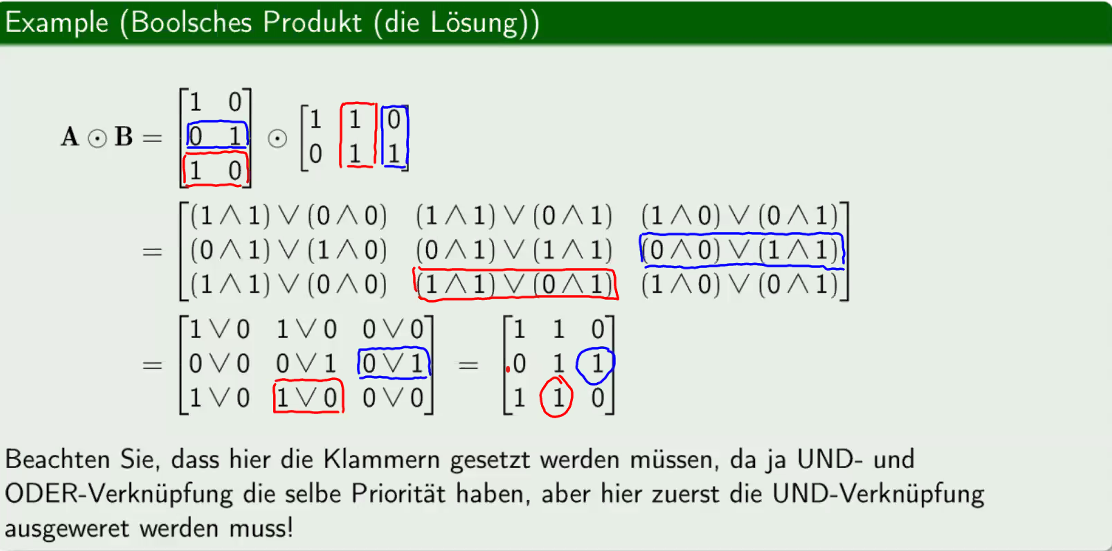
\includegraphics[width=15cm]{img/boolesches_produkt.png}

Eine quadratische Matrix kann auch eine Potenz haben:\\
$\mathbf{A}^{[r]} = \mathbf{A} \odot \mathbf{A} \dots \odot \mathbf{A}$:\\

\renewcommand{\arraystretch}{1}
$\mathbf{A} = 
\begin{bmatrix}
    0 & 0 & 1\\
    1 & 0 & 0\\
    1 & 1 & 0
\end{bmatrix}\quad\quad \mathbf{A}^2 = \mathbf{A} \odot \mathbf{A} = 
\begin{bmatrix}
    0 & 0 & 1\\
    1 & 0 & 0\\
    1 & 1 & 0
\end{bmatrix} 
\odot
\begin{bmatrix}
    0 & 0 & 1\\
    1 & 0 & 0\\
    1 & 1 & 0
\end{bmatrix}$

\newpage
\section{Mathematisches Begründen}
Bekannte Beweismethoden:
\begin{itemize}
    \item \textbf{Direkter Beweis:} Man zeigt, dass $p \rightarrow q$ wahr ist.
    \item \textbf{Beweis durch Kontraposition:} Man verwendet, dass $p \rightarrow q$ äquivalent ist zur Kontraposition
            $\lnot q \rightarrow \lnot q$.
    \item \textbf{Beweis durch Widerspruch:} Wir möchten zeigen, dass $p$ wahr ist indem\dots
\end{itemize}


\subsection{Mathematische Induktion}

\begin{enumerate}
    \item \textbf{Induktionsverankerung:} Für die kleinste Zahl zeigen, dass die Formel wahr ist (1 bei $n \in \mathbb{N}$).
    \item \textbf{Induktionsschritt:} Es wird gezeigt, dass die Implikation $P(k) \rightarrow P(k+1)$ wahr ist $\forall k \geq 1$.
\end{enumerate}

Beispiel: Dominosteine $\rightarrow$ falls der erste fällt, muss der 2. auch fallen. Falls der 2.
fällt muss der 3. auch fallen.\\

\textbf{Hinweis:} Immer zuerst überlegen was am Schluss herauskommen sollte, falls der Beweis mit Induktion
bewiesen werden kann, dann fällt auch das Beweisen leichter.


\subsection{Rekursiv definierte Funktionen}
Wenn eine Funktion mit Definitionsbereich $D(f) = \mathbb{N}$ für die f(0) definiert ist und
bei welcher f(k) durch f(k-1), f(k-2) \dots f(1), f(0) berechnet wird.
\textbf{Beispiel:} Fibonacci Folge.\\

Diese kann man auch mit Induktion beweisen.


\subsection{Beispiel Türme von Hanoi}
Vermutung: $f(n) = 2^n - 1$\\
Das heisst $f(n+1) = 2^{n+1} - 1$\\


$f(1) = 2 - 1 = 1$: stimmt\\
Es braucht $2^n$ Züge um einen Turm zu bewegen.\\
Dann brauch es +1 um die unterste Scheibe (n+1 Scheibe) zu verschieben.\\
Und schlussendlich noch einmal $2^n + 1$\\
Das ergibt: $2* (2^n-1) + 1 = 2^{n+1} - 2 + 1 = 2^{n+1} - 1$ \\
\underline{Vermutung stimmt.}

\section{Grundlagen des Zählens}
\subsection{Zusammenfassung}
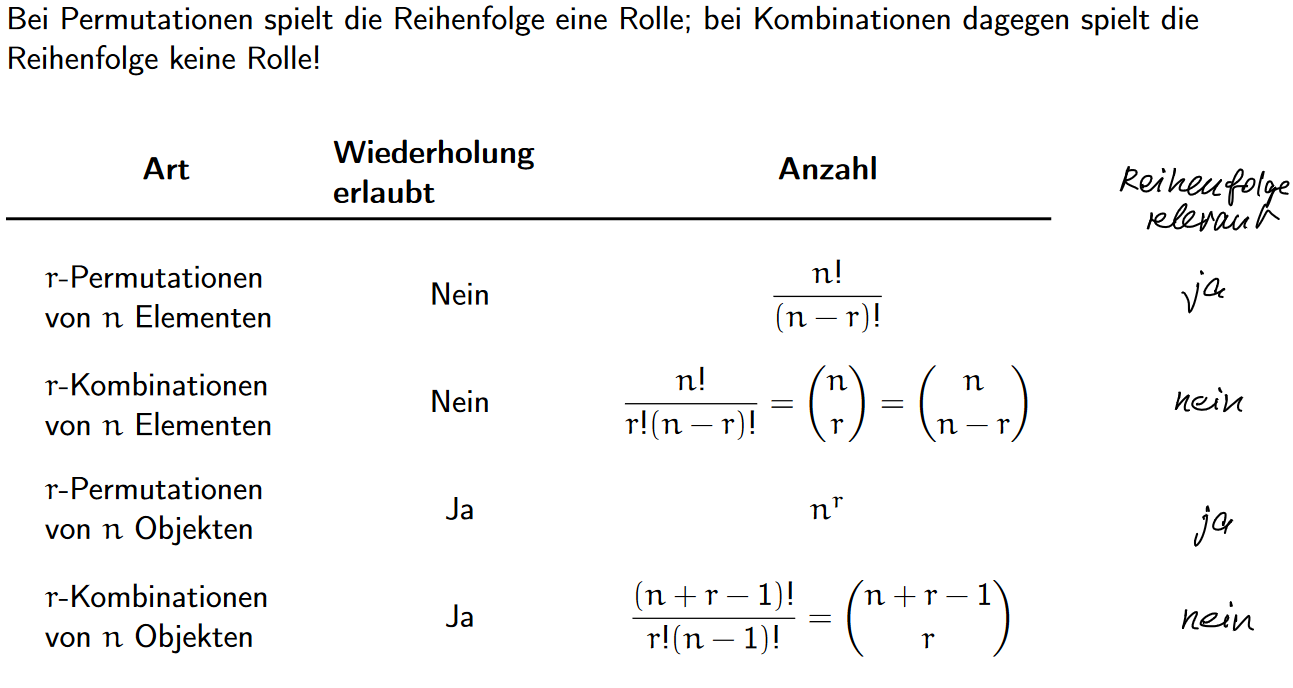
\includegraphics[width=15cm]{img/wahrscheinlichkeiten.png}


\subsection{Schubfachprinzip}
Es gibt wenigstens ein Fach in das mehr als 2 Objekte reingehen.\\

\textbf{Beispiel:} In jeder Menge von 5 Zahlen gibt es 2, welche bei einer
Division durch 4 den gleichen Rest geben.\\
Bei einer Divison durch 4 gibt es Reste von 0, 1, 2 oder 3. Man hat 5 Zahlen, heisst
2 Zahlen müssen sich denselben Rest teilen.\\


\newpage 
\subsection{Permutationen}
Eine Permutation von $n$ verschiedenen Elementen ist eine geordnete Anordnung dieser $n$ Elemente.\\
Das heisst die Anordnung (3,1,2) der Menge S={1,2,3} ist eine Permutation von $S$.\\
3-Permutationen ((1,2,3), (1,3,2), (2,1,3), (2,3,1), (3,1,2), (3,2,1)): 3!\\
2-Permutationen ((1,2), (1,3), (2,1), (2,3), (3,1), (3,2)): $2 \cdot 3$\\

Allgemeine Formel für Anzahl r-Permutationen einer Menge von n Elementen:\\

\[P(n, r) = \frac{n!}{(n-r)!}\text{, } \quad 0 \leq r \leq n \in \mathbb{N}\]

n = die Anzahl Elemente\\
r = die Anzahl Elemente im Tuple\\

Die Reihenfolge \textbf{spielt} eine Rolle.


\subsection{Permutation nicht unterscheidbarer Objekte}
Die Anzahl verschiedener Permutationen von n Objekten, von denen $n_1$ Objekte der Art 1, $n_2$ Objekte der Art 2, 
\dots, $n_k$ Objekte der Art k sind, ist gegeben durch:

\[\frac{n!}{n_1!n_2! \dots n_k!} \text{, wobei } n = \sum_{i=1}^{k} n_i\]

\textbf{Beispiel:}\\
wie viele Wörter kann man aus den Zeichen von SUCCESS machen?\\
$n = SUCCESS = 7$\\
$n_1 = S = 3$\\
$n_2 = U = 1$\\
$n_3 = C = 1$\\
$n_4 = E = 2$\\

Ergibt: $\displaystyle{\frac{7!}{3!2!1!1!} = \frac{7!}{3 \cdot 2 \cdot 2} = 420}$


\newpage
\subsection{Kombinationen}
Für $S = \{1, 2, 3, 4\}$ ist \{1, 3, 4\} eine 3-Kombination von S. Beachte, dass \{3, 1, 4\} die selbe
3-Kombination von S ist.\\

Die Reihenfolge spielt \textbf{keine} Rolle.\\

Die Anzahl von $r$-Kombinationen einer Menge von $n \geq 0$ Elementen isst gegeben durch:

\[C(n, r) = \frac{n!}{r!(n-r)!} = \binom{n}{r} = C(n, n-r)\]

n = die Anzahl Elemente\\
r = die Anzahl Elemente im Set\\




\subsection{Kombinationen mit Wiederholungen}
\textbf{Beispiel:} Wie viele verschiedene Früchteschalen kann man mit Äpfeln, Orangen und Birnen
machen, wenn immer 4 Früchte verwendet werden?\\
AAAA, AAAO, AAAB, AAOO, AAOB \dots\\

\[C(n+r-1, r) = \binom{n+r-1}{r}\]


\subsection{Beispiel mit Autonummer}
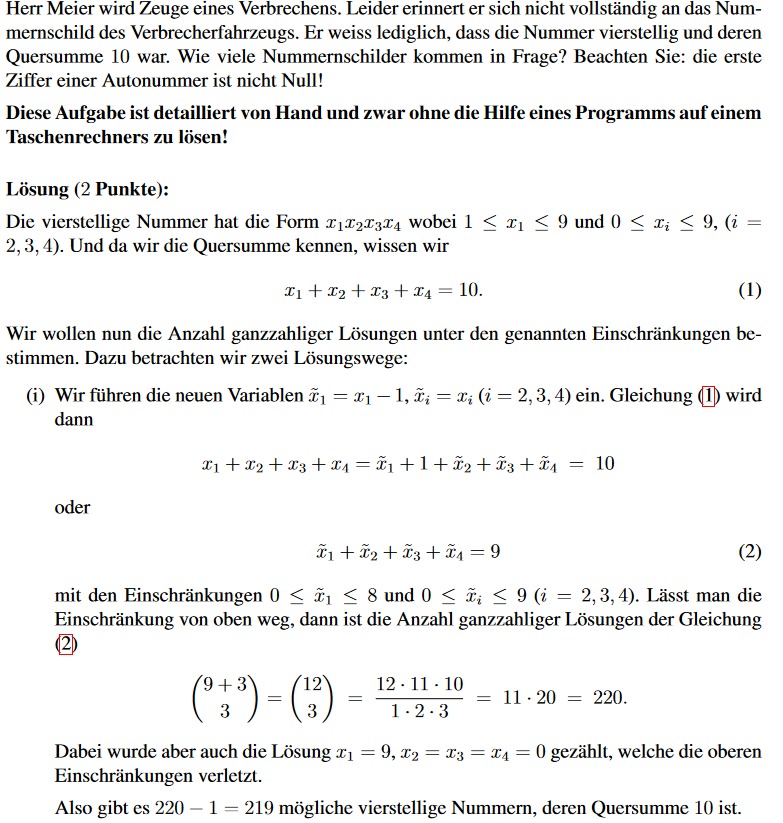
\includegraphics[width=14cm]{img/autonummer beispiel.png}


\newpage
\section{Diskrete Wahrscheinlichkeitsrechnung}
\subsection{Allgemein}

Wahrscheinlichkeiten werden oft mit $p(A)$ angegeben. Wobei $p$ die Wahrscheinlichkeit allgemein
beschreibt und $A$ der Output. Heisst $p(A)$ ist die Wahrscheinlichkeit mit der das Ereignis $A$ 
eintrifft.\\

Bezeichnungen:
\begin{itemize}
    \item $p(A|B)$: bedingte Wahrscheinlichkeit von A unter der Bedingung B
    \item $p(A \cap B)$: gemeinsame Wahrscheinlichkeit von A und B
    \item $p(B)$: bedingende Wahrscheinlichkeit von B
    \item $\Omega$: Stichprobenraum (bei Münze ist $\Omega = \{K, Z\}$)
    \item E: mögliches Ereignis. $E \subset \Omega$ oder $E = \{K, Z\}$
\end{itemize}

Beispiel:\\
Bei einem Würfel ist ein Ereignis eine ungerade Zahl zu würfeln: $E = \{1, 3, 5\} \subset \Omega$\\

Die Wahrscheinlichkeit, dass Ereignis $A$ eintrifft, ist gegeben durch $p(A)$.\\
$\displaystyle{p(A) = \frac{\vert A \vert}{\vert \Omega \vert} = \frac{\text{Anzahl günstige Fälle}}{\text{Anzahl mögliche Fälle}}}$\\


\subsection{Bedingte Wahrscheinlichkeit}
\textbf{Definition:} Die Wahrscheinlichkeit, dass ein Erei0gnis A eintritt, wenn ein Ereignis B eingetreten ist, ist gegeben durch\\
$p(A|B) = \frac{p(A \cap B)}{p(B)}$ (siehe Beispiel mit Münze in SW06). \\

Falls $A_1$ und $A_2$ zwei Ereignisse desselben Stichprobenraumes sind, dann gilt:\\
$p(A_1 \cup A_2) = p(A_1) + p(A_2) - p(A_1 \cap A_2)$\\
Zum Beispiel: ``ist eine Zahl durch 2 oder 3 teilbar?''\\

Zwei Ereignisse $A$ und $B$ sind unabhängig, wenn gilt:\\
$p(A \cap B) = p(A) \cdot p(B)$ resp.\\
$p(A|B) = p(A)$\\


\newpage
\subsection{Totale Wahrscheinlichkeit}
Wenn zwei Mengen komplementierend sind ($B$ und $\overline{B}$, z.B. lange und kurze Schrauben in Schachtel), 
dann gilt:\\
$p(A) = p(A|B) \cdot p(B) + p(A|\overline{B}) \cdot p(\overline{B})$\\

Oder allgemeiner (z.B. wenn Schrauben auf mehrere Schachteln verteilt sind):\\

$\displaystyle{p(A) = \sum_{i=1}^{n} p(A|B_i) \cdot p(B_i)}$\\

Wobei dann $B_i$ jeweils die einzelnen Schachteln wären und $p(A|B_i)$ die Wahrscheinlichkeit in der 
jeweiligen Schachtel.\\

Wenn es noch eine Bedingung $C$ gibt, dann gilt:\\
$\displaystyle{p(A) = \sum_{i=1}^{n} p(A|B_i \cap C) \cdot p(B_i|C)}$\\


\newpage
\subsection{Satz von Bayes}
Bei zwei ergänzenden Mengen:\\
\begin{align*}
    p(B|A)  &= \frac{p(A|B) \cdot p(B)}{p(A)} \\
            &= \frac{p(A|B) \cdot p(B)}{p(A|B) \cdot p(B) + p(A|\overline{B}) \cdot p(\overline{B})}\\
\end{align*}

\textbf{Beispiel:}\\
$0.5\%$ haben Krankheit. Test ist bei Kranken zu $99\%$ korrekt. Test gibt
aber auch bei $2\%$ Gesunden an. Wenn Test positiv, wie gross ist die Wahrscheinlichkeit,
dass Person effektiv krank ist?

\begin{itemize}
    \item Kranke: $K$
    \item Gesunde: $\overline{K}$
    \item Test positiv: $T$
    \item Test negativ: $\overline{T}$
\end{itemize}

$p(K) = \frac{5}{1000}$ und $p(\overline{K}) = \frac{995}{1000}$\\
$p(T|K) = \frac{99}{100}$ und $p(T|\overline{K}) = \frac{2}{100}$\\

Durch Satz von totaler Wahrscheinlichkeit:\\
$p(T) = p(T|K) \cdot p(K) + p(T|\overline{K}) \cdot p(\overline{K}) = \frac{5}{1000} \cdot \frac{99}{100} + \frac{995}{1000} \cdot \frac{2}{100} = \frac{497}{20000}$\\


Dann mit Satz von Bayes:\\
\begin{align*}
 p(K|T) &= \frac{p(T|K) \cdot p(K)}{p(T)} \\
        &= \frac{\frac{99}{100} \cdot \frac{5}{1000}}{\frac{99}{100} \cdot \frac{5}{1000} + \frac{2}{100} \cdot \frac{995}{1000}} \\
        &= \frac{\frac{99}{100} \cdot \frac{5}{1000}}{\frac{497}{20000}} \\
        &= \frac{495}{2485} \approx 0.2\\
\end{align*}

\newpage
\subsection{Verteilungsfunktionen}

\vspace{0.5cm}
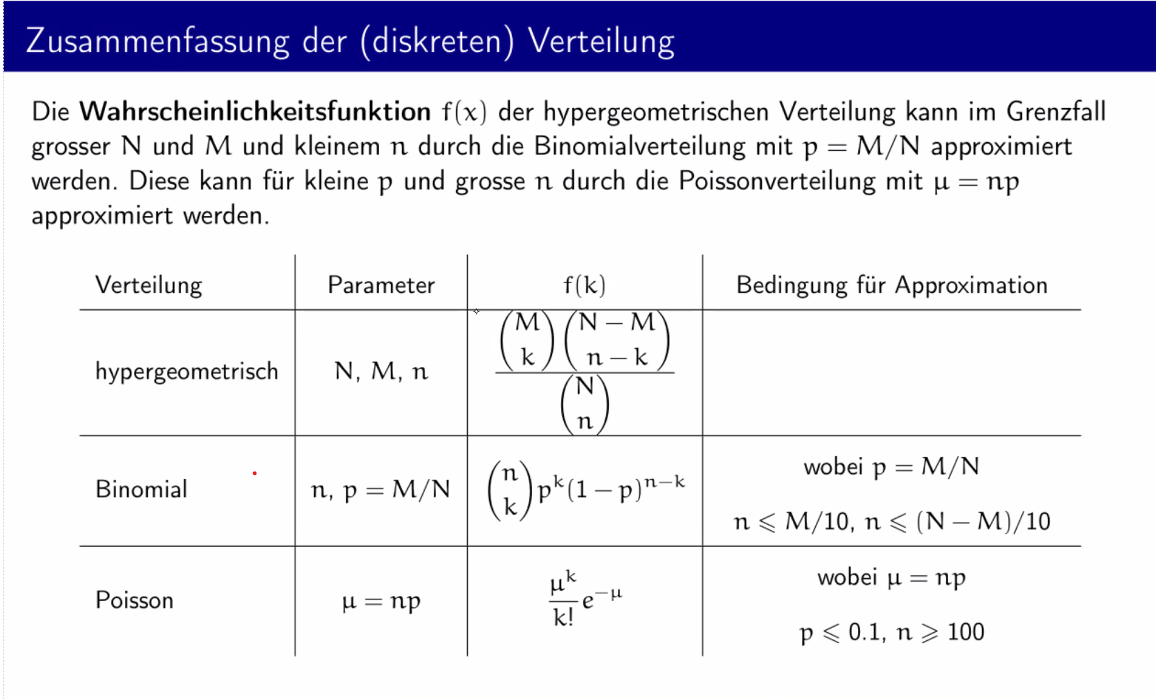
\includegraphics[width=15cm]{img/zusammenfassung _verteilungen.png}

\subsubsection{Bernoulli-Verteilung}
Zufallsexperiment mit nur 2 möglichen Ergebnissen, wobei die Bernoulli-Verteilung der 
Wahrscheinlichkeitsverteilung entspricht. Wobei wahr p entspricht und falsch 1-p.
Die Wahrscheinlichkeiten müssen dabei voneinander unabhänig sein.\\

\textbf{Beispiel:}
Bitstring mit 3 Bits bei der n-Einsen vorkommen (und wenn man eine 1 Würfelt ist es ein
Erfolg resp. $p$ oder ein nicht-Erfolg resp. $1-p$ oder $q$).\\

P(k=0) = P(\{000\}) = $1p^0 \cdot (1-p)^3$\\
P(k=1) = P(\{001\},\{010\},\{010\}) = $3p^1 \cdot (1-p)^2$\\
P(k=2) = P(\{011\},\{110\},\{101\}) = $3p^2 \cdot (1-p)^1$\\
P(k=3) = P(\{111\}) = $1p^3 \cdot (1-p)^0$\\

\textbf{Definition durch Binomialverteilung:}\\
$B(k|n,p) = B_{n,p}(k) = C(n,k)p^k(1-p)^{n-k} = \binom{n}{k}p^k(1-p)^{n-k}$\\
B: Bernoulli\\
k: Anzahl Erfolge\\
n: Anzahl Versuche\\
p: Wahrscheinlichkeit für Erfolg bei einem Wurf\\

Mit dieser Formel kann man die Wahrscheinlichkeit ausrechnen für k-Erfolge.\\


\textbf{Beispiel für eine Ungleichverteilung:}\\
Eine 0 wird zu 90\% und eine 1 zu 10\% gewürfelt. Wie wahrscheinlich ist es 8 Nullen bei
10 Würfen zu erzielen.\\

$B(8|10,0.9) = \binom{10}{8} \cdot 0.9^8 \cdot 0.1^2 = 19.37\%$

\subsubsection{Hypergeometrische Verteilung}
Binomialverteilung liegt vor, wenn bei einer Stichprobe die Objekte wieder zurückgelegt werden.
Werden die Objekte nicht wieder zurückgelegt handelt es sich um die Hypergeometrische Verteilung.\\

\textbf{Beispiel:}\\
Wenn man insgesamt N Objekte hat und M davon sind defekt. Wie gross ist die Wahrscheinlichkeit,
dass von n gezogenen Objekten k Objekte defekt sind?\\

$\displaystyle{p(k) = \frac{\binom{M}{k} \binom{N-M}{n-k}}{\binom{N}{n}}}$\\
\vspace{1cm}


\textbf{Anschauliches Beispiel:}\\
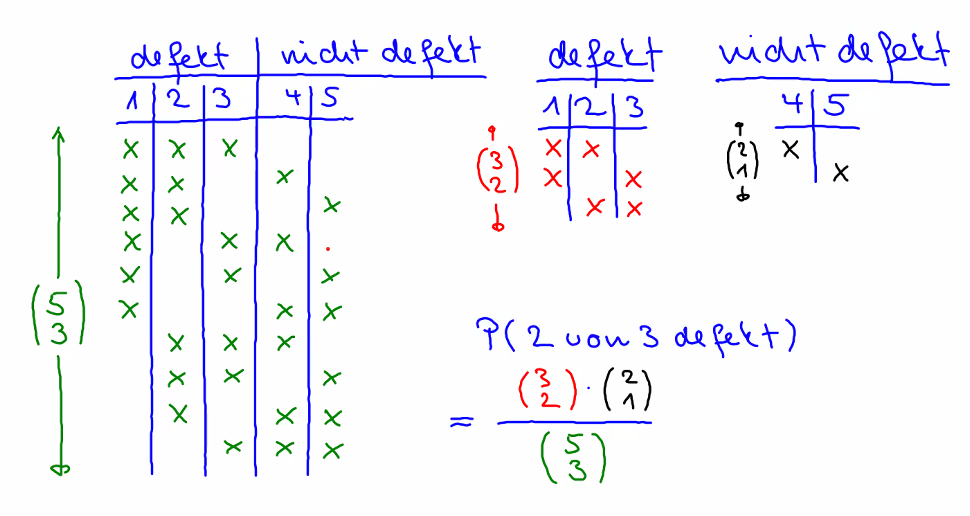
\includegraphics[width=15cm]{img/hypergeometrische Verteilung.png}

Grün: Anzahl der Objekte\\
Rot: Anzahl der Objekte die defekt sind\\
Schwarz: Anzahl der Objekte die nicht defekt sind\\


\subsubsection{Poisson-Verteilung}
Wenn bei einer Binomialverteilung sehr viele Versuche durchgeführt werden und die Wahrscheinlichkeit 
sehr klein ist, ist die Annäherung durch die Poisson-Verteilung viel einfacher.\\
$p \rightarrow 0$ und $n \rightarrow \infty$ dann $\mu = np$:\\

$\displaystyle{p(k) = \frac{\mu^k e^{-\mu}}{k!}}$\\


\subsection{Zufallsvariablen}
Wahrscheinlichkeitsverteilung einer Zufallsvariable $X$ auf einem Stichprobenraum
$S$ ist die Menge\\

$\{(r,p(X=3))\} | \forall r \in X(S)$

Wobei $p(X=3)$ die Wahrscheinlichkeit dafür ist, dass die Zufallsvariable $X$ den Wert $r$
annimmt.\\

\textbf{Beispiel:}\\
Münze wird 3-mal geworfen. Wie oft hat sie eine 1 gezeigt?\\

\renewcommand{\arraystretch}{1.5}
\begin{center}
    \begin{tabular}{ | c | c | c | c | c |}
        \hline
        $r$ & 0 & 1 & 2 & 3\\ 
        \hline
        $p(X=r)$ & $\frac{1}{8}$ & $\frac{3}{8}$ & $\frac{3}{8}$ & $\frac{1}{8}$\\ 
        \hline
    \end{tabular}
\end{center}


\newpage
\subsection{Erwartungswert einer Zufallsvariablen}
Erwartungswert einer Zufallsvariable $X(s)$ von Stichprobenraumm $S$:\\

$\displaystyle{E(X) = \sum_{r \in X(S)} r \cdot p(X=r)}$\\

\textbf{Beispiel:}\\
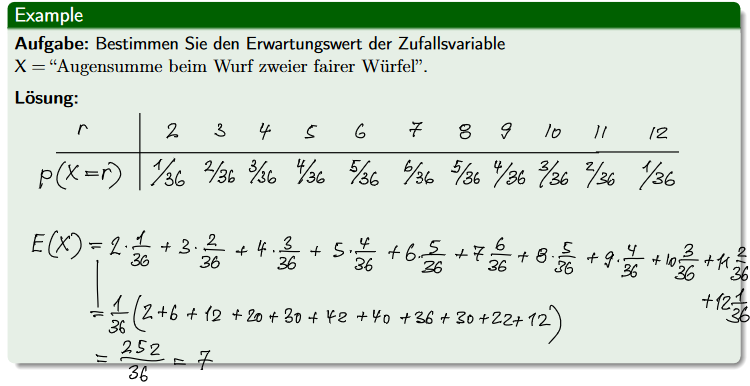
\includegraphics[width=14cm]{img/erwartungswert_zufallsvariable.png}\\

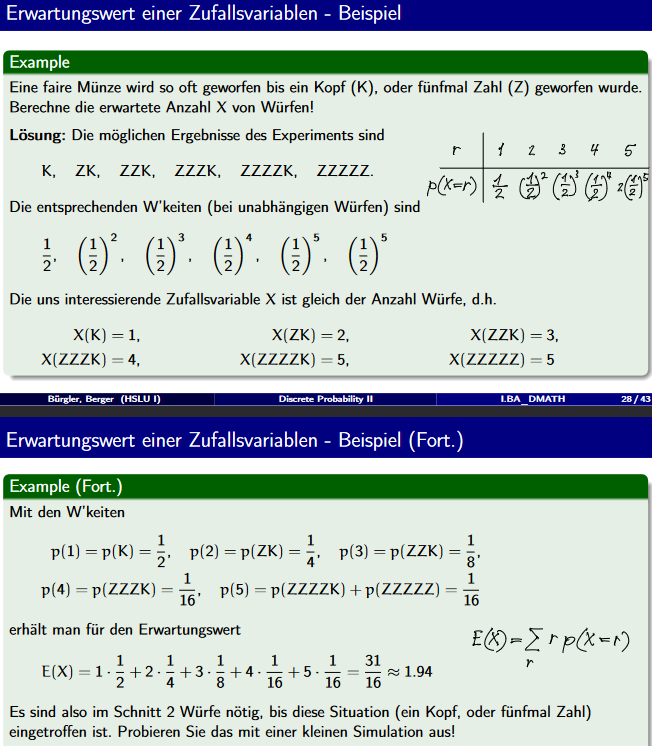
\includegraphics[width=14cm]{img/erwartungswert_zufallsvariable2.png}

\newpage
\section{Fortgeschrittene Zählmethoden}
\subsection{Rekursionsbeziehungen}
Rekursionsbeziehungen liegen immer vor, wenn ein Wert $a_n$ von einem anderen Wert $a_{n-1}$ abhängt.\\
Beispiel für Rekursionsbeziehungen:\\
Wie viele Bitstrings der Länge $n$ gibt es, die keine zwei aufeinanderfolgende
Nullen enthalten?\\

$a_n = a_{n-1} + a_{n-2}$\\

Ein Bitstring endet mit einer 1 oder 0. Im ersten Fall kann irgendein Wert davor stehen, davon
gibt es $a_{n-1}$ Möglichkeiten. Im zweiten Fall muss ein 1 vor der 0 stehen, davon gibt es $a_{n-2}$ Möglichkeiten.\\


\textbf{Beispiel Computersystem Passwort:}\\
Ein Passwort ist korrekt, wenn es eine gerade Anzahl von Nullen hat.\\

$a_{n-1}$ Möglichkeiten bei einer Zahl, welche mit 1-9 endet.\\
Wenn eine Null steht, dann noch $10^{n-1} - a_{n-1}$ Möglichkeiten.\\

$a_n = 9 \cdot a_{n-1} + 10^{n-1} - a_{n-1}$\\
$a_n = 8 \cdot a_{n-1} + 10^{n-1}$\\

\begin{itemize}
    \item Sie ist homogen, falls $r(n) = 0$
    \item Sie ist linear, falls die Variablen von F $a_n$, $a_{n-1}$, $a_{n-2}$ sind.
    (meistens ist F von der Form $a_n - c_1a_{n-1} - c_2a_{n-2} - \dots - c_ka_{n-k} = 0$)
    \item Sie ist von k-tem Grade, falls F höchstens von Gliedern ab $a_{n-k}$ abhängt.
\end{itemize}

\newpage
\subsection{Lösen von Rekursionsbeziehungen}
\textbf{Eigenschaften von Rekursionsbeziehungen:}\\
$F(a_n, a_{n-1} \dots a_2, a_1) = r(n)$\\

Allgemeines Lösen einer linearen RB in drei Schritten:
\begin{enumerate}
    \item Bestimme die allgemeine Lösung $\displaystyle{\left\{a_n^{(h)}\right\}}$ der zugehörigen, homogenen
    Rekursionsbeziehung (RHS gleich null setzen).
    \item Bestimme eine (einzige) partikuläre Lösung $\displaystyle{\left\{a_n^{(p)}\right\}}$ der zugehörigen, inhomogenen Rekursionsbeziehung
    \item Dann ist die allgemeine Lösung der inhomogenen RB die Summe der beiden Lösungen:
    \[\{a_n\} = \left\{a_n^{(h)}\right\} + \left\{a_n^{(p)}\right\}\]
\end{enumerate}

\textbf{1. Schritt:}

Die homogene RB\\
($a_n - c_1a_{n-1} - c_2a_{n-2} - \dots - c_ka_{n-k} = 0$)\\
wird durch den folgenden Ansatz gelöst:\\
$a_k = r^k$, $k = n-k$, $n-k + 1$, \dots, $n$.\\


\textbf{Beispiel:}

Setzt man in die lineare, homogene Rekursionsbeziehung $a_n - a_{n-1} - a_{n-2} = 0$
den Ansatz $a_n = r^n$ ein, erhält man\\

$r^n - r^{n-1} - r^{n-2} = 0$\\
$r^{n-2} (r^2 - r - 1) = 0$\\
$r^2 - r - 1 = 0$\\

$\displaystyle{r_1 = \frac{1}{2} \left(1 + \sqrt{5}\right)} \quad\quad\quad r_2 = \frac{1}{2} \left(1 - \sqrt{5}\right)$\\


Bei Auflösung der quadratischen Gleichung: \\
Wenn $D > 0$, dann $a_n^{(h)} = \alpha_1 r_1^n + \alpha_2 r_2^n$
wobei die Alphas beliebige Konstanten sind.\\

Wenn $D = 0$, dann $a_n^{(h)} = (\alpha_1 + \alpha_2 n) r^n$

\newpage
\section{Zahlentheorie}
Wiederholung:
\subsection{Modulare Arithmetik}
Zwei ganze Zahlen a und b sind kongruent modulo m, falls $m\mid (a - b)$.
Das heisst a und b liegen ein Vielfaches von m auseinander. Man schreibt dann $a \equiv b$ mod $m$ und sagt:
``a ist kongruent zu b modulo m''.\\

$13 \equiv 1$ mod 4 denn $4 \mid (13 - 1)$\\
$13 \equiv 1$ mod 3 denn $3 \mid (13 - 1)$\\
$13 \not\equiv  1$ mod 5 denn $5 \nmid (13 - 1)$\\

\subsection{Lösung diophantischer Gleichungen}
$n_1 \cdot x + n_2 \cdot y = n$\\
Hat immer dann ganzzahlige Lösungen, wenn ggT($n_1$, $n_2$) $\vert$ $n$ ist. \\Das heisst, 
falls ggT($n_1$, $n_2$) ein Teiler von $n$ ist.\\
Sind $n_1$ und $n_2$ teilerfremd, dann hat die Gleichung immer eine Lösung.\\

Kann man mit erweitertem Euklid lösen (Wiederholung):\\

\textbf{Der Euklidische Algorithmus}
Effiziente Methode um ggT zu finden.

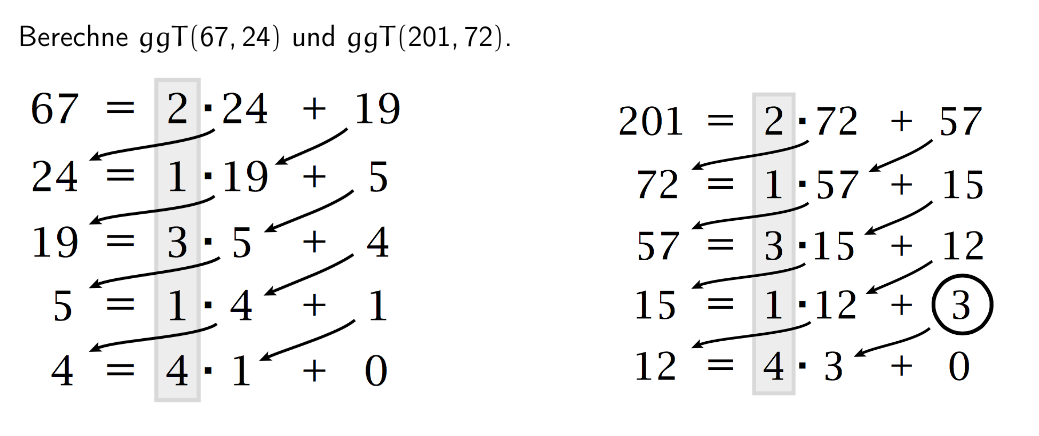
\includegraphics[width=15cm]{img/euqlidic_algorithm.png}

ggT ist jeweils 1 und 3.

\textbf{Erweiterter euklidischer Algorithmus}
Lösung der Gleichung mit der diophantischen Gleichung.\\

Finde $x$,$y \in \mathbb{Z}$ mit $211 \cdot x + 13 \cdot y = 1$\\ 

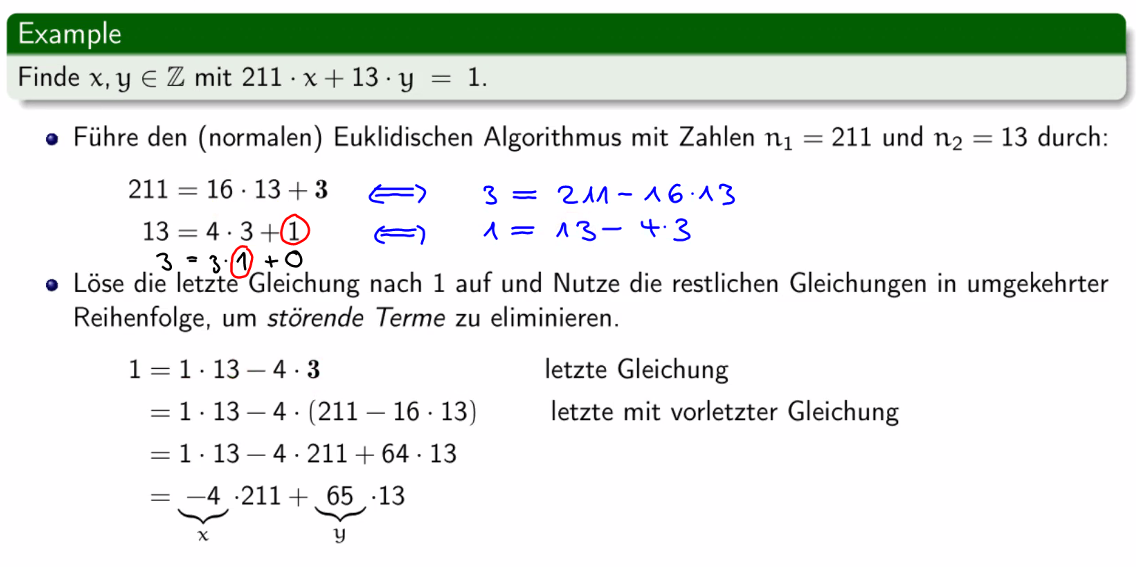
\includegraphics[width=14cm]{img/erweiterter_euklidischer_algorithmus.png}

Mit einem nächsten Beispiel: zuerst (blau) der normale euklidische Algorithmus machen
und danach der erweiterte machen (rot) von unten nach oben. Dann hat man am Schluss
x und y in der Gleichung.

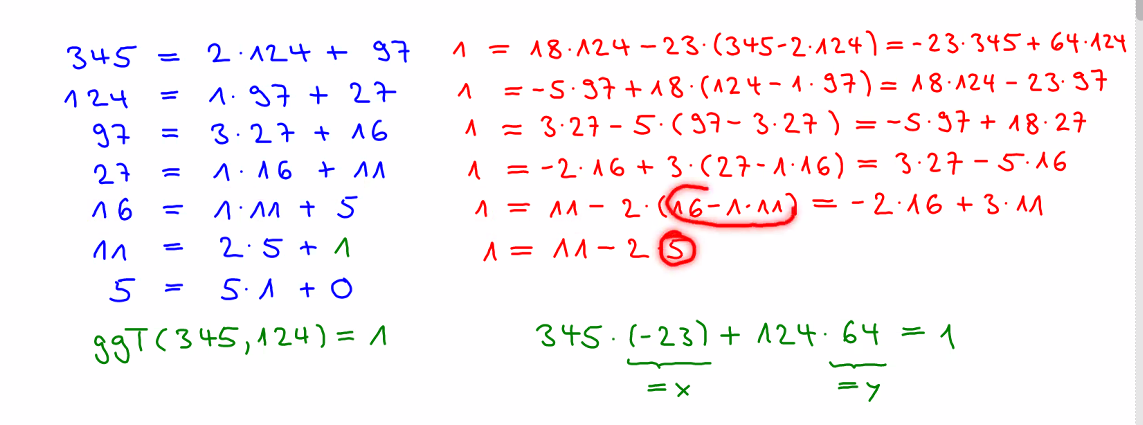
\includegraphics[width=14cm]{img/erweiterter_euklidischer_algorithmus_beispiel2.png}

Ein weiteres Beispiel:\\
Bestimme eine Zahl $x$ für die gilt: $329 \cdot x \equiv 1$ mod 587\\

Euklidischer Algorithmus:\\
\begin{align*}
    587 &= 1 \cdot 392 + 195 \\
    392 &= 2 \cdot 195 + 2 \\
    195 &= 97 \cdot 2 + 1 \\
\end{align*}

\newpage
Erweiterter euklidischer Algorithmus:\\
\begin{align*}
    1   &= 195 - 97 \cdot 2 \\
        &= 195 - 97 \cdot (392 - 2 \cdot 195)\\
        &= 195 - 97 \cdot 392 + 194 \cdot 195\\
        &= 195 \cdot 195 - 97 \cdot 392\\
        &= 195 \cdot (587 - 392) - 97 \cdot 392\\
        &= 195 \cdot 587 - 292 \cdot 392\\
\end{align*}

$1 \equiv \mathbf{292} \cdot 392$ mod $587$\\

\subsection{Modulare Inverse}
x mal was gibt 1: $3^{-1} \cdot \frac{1}{3} = 1$\\

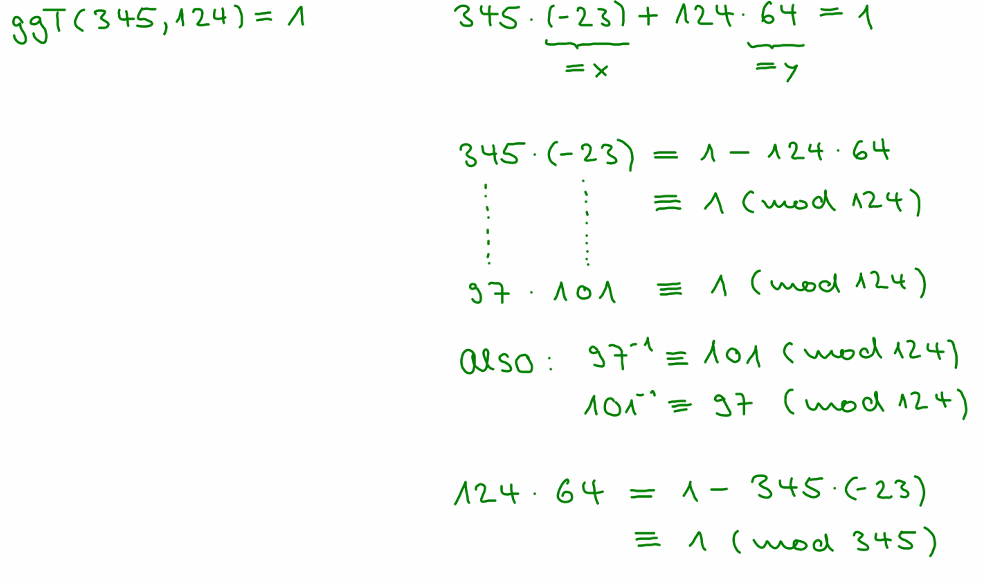
\includegraphics[width=14cm]{img/modulo inverse_beispiel.png}


Das heisst, dass wo immer eine 1 in der Grafik ist, existiert ein modulo inverse.
Ist die Modulo Zahl eine Primzahl existiert immer ein modulo inverse, andererseits nicht unbedingt.\\

Grundsätzlich mit erweitertem euklidischem Algorithmus lösen.\\


\subsection{Der chinesische Restsatz}
Seien $m_1,m_2, \dots, m_k$ paarweise teilerfremde Zahlen. Dann hat das System k simultane Kongruenzen\\

\begin{align*}
    x &\equiv r_1 \mod m_1 \\
    x &\equiv r_2 \mod m_2 \\
    \vdots \\
    x &\equiv r_k \mod m_k \\
\end{align*}

\textbf{Konstruktionskonzept:}\\
$m = m_1 \cdot m_2 \cdots m_k$
\begin{enumerate}
    \item Dann definieren wir für alle $i = 1,2, \dots, k$:\\
 
    $\displaystyle{M_i = \frac{m}{m_i}}$\\

    Sicher gilt dann ggT($m_i$, $M_i$) = 1. Denn die Voraussetzung ist, dass alle $m_i$ teilerfremd sind.\\
    \item Für $i = 1,2,\dots k$ hat $M_i$ ein modulares Inverses (erweiterter euklidischer Algorithmus)
    $y_i$ modulo $m_i$, d.h.\\

    $\displaystyle{M_i \cdot y_i \equiv 1}$ (mod $m_i$)\\

    \item Die simultane Lösung der Kongruenzen ist dann:\\
    
    $\displaystyle{x = \sum_{i=0}^{k} r_i \cdot M_i \cdot y_i}$\\

\end{enumerate}


\newpage
\subsection{Eulersche $\phi$-Funktion}
Allgemein Mengen:\\
$\mathbb{Z}_n := \{0,1,2,3, \dots, n-1\}$, wobei $|\mathbb{Z}_n| = n$, das heisst: $\mathbb{Z}_4 = \{0, 1, 2, 3\}$ und $|\mathbb{Z}_4| = 4$\\
$\mathbb{Z}_n^* := $ beschreibt alle Elemente kleiner $n$, welche teilerfremd zu $n$ sind\\

Mit der eulerschen $phi$-Funktion kann man berechnen wie viele Elemente in $\mathbb{Z}_n^*$ enthalten sind.\\


\subsection{Eigenschaften der Eulerschen $\phi$-Funktion}
Vorausgesetzt: $p$ und $q$ sind zwei verschiedene Primzahlen und $m$ ist eine natürliche Zahl mit der Primfaktorzerlegung:\\

$m = p_1^{r_1} \cdot p_2^{r_2} \cdots p_n^{r_n}$\\

und $n$ ist eine natürliche Zahl und teilerfremd zu $m$\\

Dann gilt:

\begin{align*}
    \phi(p) &= p - 1 \\
    \phi(p \cdot q) &= (p - 1) \cdot (q - 1) \\
    \phi(m) &= (p_1 - 1) \cdot p_1^{r1-1} \cdot (p_2 - 1) \cdot p_2^{r_2 - 1} \cdots (p_n - 1) \cdot p_n^{r_n - 1} \\
    \phi(m \cdot n) &= \phi(m) \cdot \phi(n) \\
\end{align*}

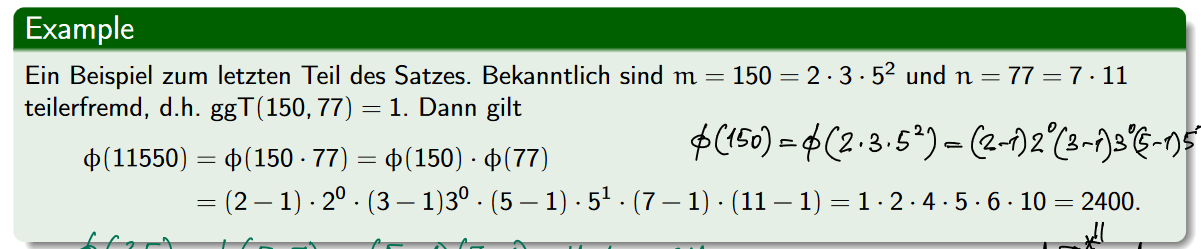
\includegraphics[width=14cm]{img/example_euler_phi.png}

\newpage
\subsection{Der kleine Satz von Fermat}
Sei $p$ eine Primzahl und $m$ eine nicht negative Zahl, dann gilt:\\

$m^p \mod p = m \mod p$\\


\subsection{Der Satz von Wilson}
Eine natürliche Zahl $n > 1$ ist genau dann eine Primzahl, wenn\\
$(n-1)! + 1$ durch $n$ teilbar ist.\\



\subsection{Relationen}
Eine Relation R auf einer Menge $A$ ist eine Teilmenge von $A \times A$.\\

$\{1,2,3\}^2 = $
\begin{align*}
    \{ &(1,1), (1,2), (1,3) \\
       &(2,1), (2,2), (2,3) \\
       &(3,1), (3,2), (3,3)\} \\
\end{align*}

$R$ ist zum Beispiel = $\{(1,2), (1,3), (2,3)\}$\\

Wenn $A$ die Menge aller Landpunkte auf einem Planet ist, dann ist

$R = \{(x,y) \in A \times A | y$ lässt sich von $x$ aus trockenen Fusses erreichen\}

$R = \{(x,y) \in \mathbb{Z} \times \mathbb{Z}|y \equiv x \mod n\}$


\subsubsection{Symmetrische Relationen}
Eine symmetrische Relation ist, wenn man in der obigen Definitionsformel $x$ und $y$ vertauschen kann.\\

$\forall x,y \in A((x,y) \in R \longrightarrow (y,x) \in R)$.\\

Auf dem Planet, lässt sich von jedem Punkt zu einem Anderen auf der Landmasse der Weg umkehren (rückwärts gehen).

\newpage
\subsubsection{Transitive Relationen}
Wenn für jedes Element folgendes gilt: Wenn sich von $x$ aus $y$ erreichen lässt und von $y$ aus lässt sich $z$ erreichen, 
dann lässt sich von $z$ aus auch $x$ erreichen (ist wahr auf dem Planet, mit der Landmasse), dann ist die Relation transitiv.\\

$x,y,z \in \mathbb{Z} \text{ mit } y \equiv x \mod n$ \textbf{und} $z \equiv y \mod n$ \textbf{und} $z \equiv x \mod n$\\


\subsubsection{Äquivalenzrelationen}
\textbf{Definition:} Falls die Relation auf der Menge $A$ symmetrisch und transitiv ist, dann ist sie 
eine Äquivalenzrelation.\\

\subsection{Restklassen}
Die Restklassen sind immer die Zahlen, welche in Relation zueinander stehen (kongruent sind).\\

Alle ganzen Zahlen ergeben sich aus den Restklassen $\mathbb{Z} = [0] \cup [1] \cup \dots \cup [n-1]$ dargestellt.\\

\subsection{Modulares Rechnen}
\subsubsection{Modulare Rechenoperationen}
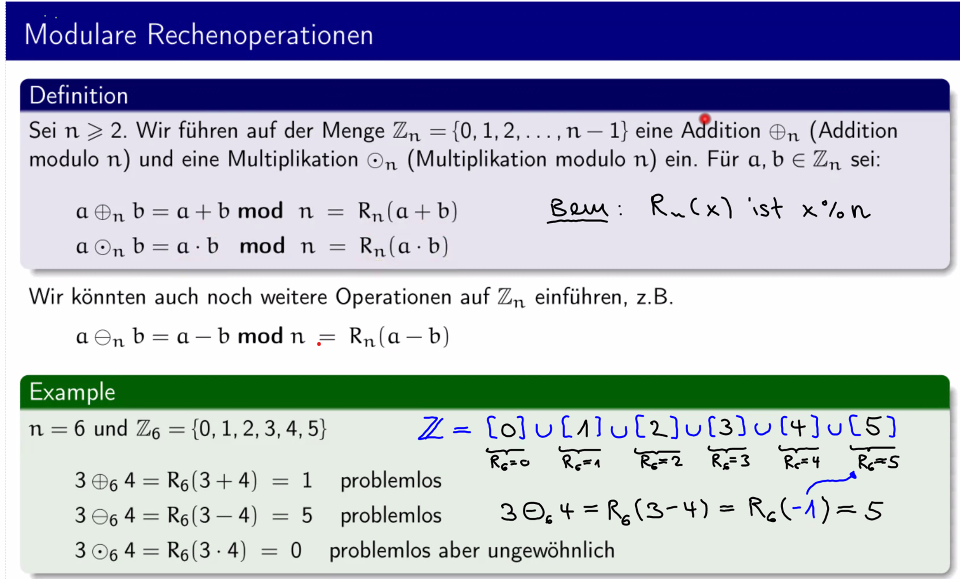
\includegraphics[width=14cm]{img/modulare_rechenoperationen.png}


\subsubsection{Modulare Rechenregeln}
Random aber wichtig:\\
$3n + 6 \mod n = (3n \mod n) + (6 \mod n)$

\vspace{0.5cm}

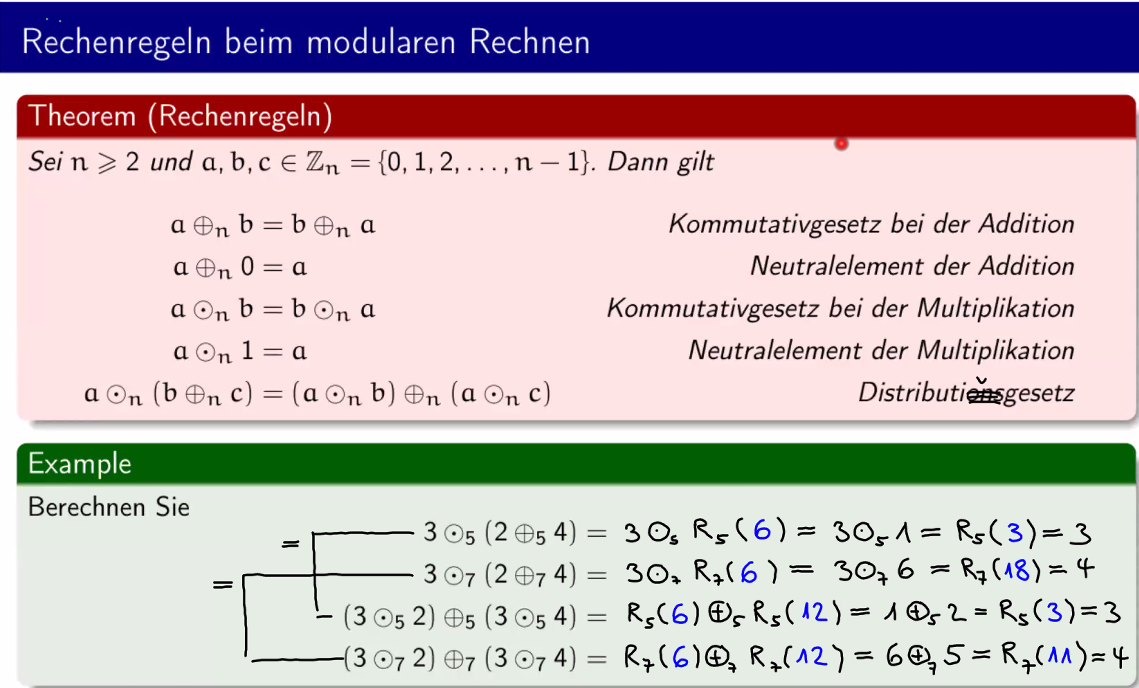
\includegraphics[width=14cm]{img/modulare_rechenregeln.png}

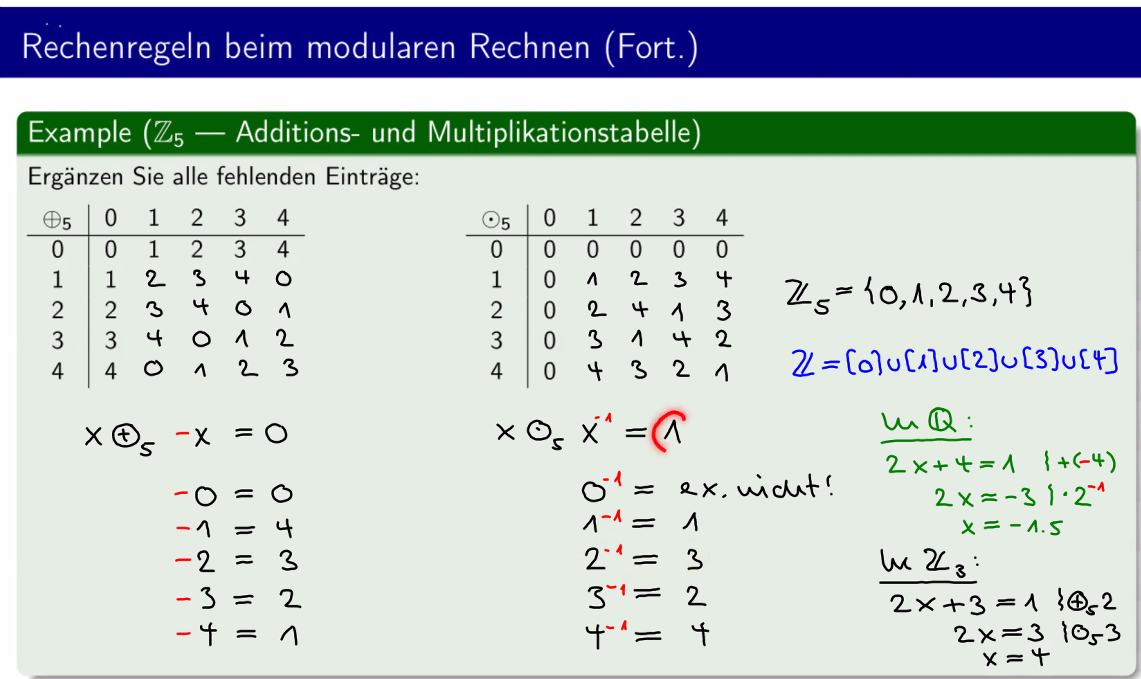
\includegraphics[width=14cm]{img/modulare_rechenregeln2.png}

\newpage
\subsection{Square-and-Multiply-Algorithmus}
Effizientes potenzieren modulo n.\\
Exponent binär schreiben und 2 nach rechts ausklammern.

\begin{align*}
    21 = (10101)_2  &= 2^4 + 2^2 + 1\\
                    &= (2 \cdot 2 + 1) \cdot 2 \cdot 2 + 1\\
\end{align*}

\begin{align*}
    5^{21} \mod 11  &= 5^{(2 \cdot 2 + 1) \cdot 2 \cdot 2 + 1} &\mod 11\\
    &= (((5^2)^2 \cdot 5)^2)^2 \cdot 5 &\mod 11\\
                    &= ((25^2 \cdot 5)^2)^2 \cdot 5 &\mod 11\\
                    &= (((25)^2 \cdot 5)^2)^2 \cdot 5 &\mod 11\\
                    &= ((3^2 \cdot 5)^2)^2 \cdot 5 &\mod 11\\
                    &= (1^2)^2 \cdot 5 &\mod 11\\
                    &= 5\\
                \end{align*}
                
Formal:\\
\begin{itemize}
    \item Q bedeutet quadrieren und M multiplizieren
    \item Ersetze in der binären Darstellung des Exponenten jede 1 durch QM und jede 0
    durch Q $(10101)_2 \rightarrow QMQQMQQM$
    \item Streiche das erste (links vorkommende) QM\\
    $QMQQMQQM \rightarrow QQMQQM$
    \item Das Symbol QQMQQM gibt die Reihenfolge von Quadrieren und Multiplizieren an, um
    um die Potenz zu berechnen. Nach jeder Operation wird das Ergebnis modulo 11 reduziert.
\end{itemize}


\textbf{Beispiel:}\\
$5^{21} \mod 11$\\
$5 \xrightarrow{Q} 25 \equiv 3 \xrightarrow{Q} 9 \xrightarrow{M} 45 \equiv 1 \xrightarrow{Q} 1 \xrightarrow{Q} 1 \xrightarrow{M} 5$\\


\newpage
\subsection{Multiplikative Inverse}
Die Euler'sche $\phi$-Funktion von $n$ gibt die Anzahl invertierbarer Element kleiner als $n$.

\subsubsection{Generell}
Jede Zahl bei welcher gilt ggT($a,n$) = 1, hat eine multiplikative Inverse.\\
Das multiplikativ Inverse kann dann mit dem erweiterten euklidischen Algorithmus berechnet werden
oder direkt aus der Tabelle herausgelesen werden.\\


\subsubsection{Mit Primzahlen}
Ist $p$ eine Primzahl, dann kann man mit dem kleinen Satz von Fermat die Inversen systematisch bestimmen.\\
In $\mathbb{Z}_p$ gilt: $a^{p-1} \equiv 1 \mod p$\\

Für jedes $0 < a < p$ gilt: $a^{p-2} \mod p$ ist das Inverse zu $a$ modulo $p$\\

\textbf{Beispiel:}\\
Das Inverse von 2 modulo 19:\\
\begin{align*}
    2^{-1}  &= 2^{19-2} \mod 19\\
            &= 2^{17} \mod 19 \rightarrow \text{use SMA}\\
            &= 10 \text{ denn } 2 \cdot 10 = 20 \equiv 1 \mod 19\\
\end{align*}

\subsection{Primitive Elemente}
Sei $p$ eine Primzahl. Ein Element $z$ von $\mathbb{Z}_p$ heisst primitiv, falls jedes Element
von $\mathbb{Z}_p$ eine Potenz von $z$ ist.\\

\textbf{Beispiel:}\\
In $\mathbb{Z}_{5}$ ist 2 ein primitives Element, denn $2^1 = 2, 2^2 = 4, 2^3 = 3, 2^4 = 1$\\

\newpage
\subsection{Einwegfunktionen}
Ein paar bekannte Einwegfunktionen:
$p$ und $q$ sind Primzahlen, $n = pq$ und $e$ ist eine Zahl mit ggT($e, \phi(n)$) = 1

\begin{itemize}
    \item $x \rightarrow x^2 \mod n$
    \item $x \rightarrow x^e \mod n$
    \item $k \rightarrow b^k \mod p$
\end{itemize}


\subsection{Modulare Quadratwurzeln}
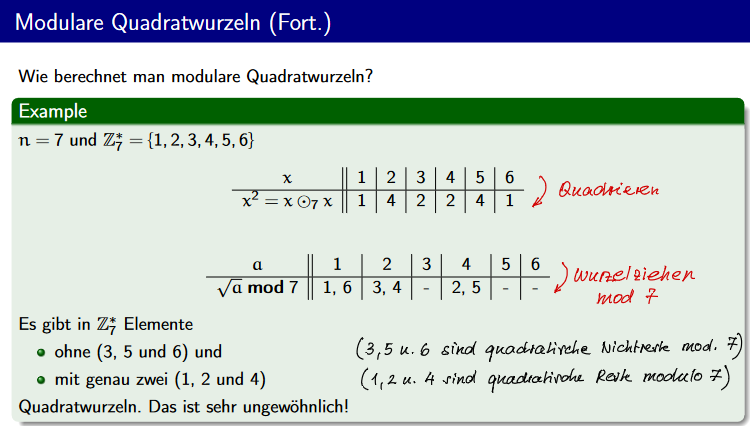
\includegraphics[width=14cm]{img/modulare_quadratwurzeln.png}


Viel einfacher mit Euler-Kriterium:\\
Wenn man wissen will ob $x$ ein qadratischer Rest (quadratisches Residuum) von
modulo $y$ ist dann rechnet man:\\
$x^{\frac{y-1}{2}} \mod y$\\
wenn Ergebnis $=1$ dann ist es ein Rest sonst nicht.\\

\textbf{Beispiel:}\\
Ist 7 ein quadratischer Rest modulo 17?\\
$7^{\frac{17-1}{2}} \mod 17 = 7^8 \mod 17 = -1 \neq 1$\\

Antwort: Nein!


\newpage
\subsection{Der diskrete Logarithmus}
$p$ ist immer eine Primzahl.\\
Die Funktion ist definiert als:\\
$y = b^k \mod p$\\

$y$ ist $\in \mathbb{Z}_p$.\\
Unter dem Problem versteht man: Finde ein $k$ für welches gilt die obige Gleichung gilt\\

\subsection{Diffie-Hellman-Schlüsselaustausch}
\begin{enumerate}
    \item Wähle zwei grosse Primzahlen $p$ und $q$ und ein $g < p$ (ist Erzeugende in $\mathbb{Z}_p$)
    \item $A$ wählt Zufallszahl $a < p$ und berechnet $\alpha = g^a \mod p$ und sendet $\alpha$ an $B$
    \item $B$ wählt Zufallszahl $b < p$ und berechnet $\beta = g^b \mod p$ und sendet $\beta$ an $A$
    \item $A$ berechnet $\beta^a \mod p$ und $B$ berechnet $\alpha^b \mod p$ und beide erhalten den gleichen Schlüssel
\end{enumerate}

\newpage
\section{Kryptografie}
\subsection{Perfekte Sicherheit}
Ein \textbf{Verschlüsselungsverfahren} ist perfekt sicher, wenn die Kenntnis eines Geheimtextes $c$ keine Information
über das Vorliegen eines Klartextes $m$ liefert.\\

Ein \textbf{Kryptosystem} heisst perfekt sicher, falls die Ereignisse, dass ein bestimmter Geheimtext c
auftritt und ein bestimmter Klartext m vorliegt, unabhängig sind, d.h. es gilt
$\forall c, \forall m (p(m \vert c) = p(m))$.\\

\subsection{Symmetrische Verschlüsselung}
Besteht immer aus folgenden Elementen:
\begin{itemize}
    \item \textbf{Schlüssel} $k \in K$ (Schlüsselraum)
    \item \textbf{Klartext} $m \in M$ (Klartextraum)
    \item \textbf{Geheimtext} $c \in C$ (Geheimtextraum) welcher sich folgendermassen ergibt:
    $c = f(k, m)$
\end{itemize}

Dabei muss immer gelten, dass $f$ eine Umkehrfunktion hat, mit welcher sich der Geheimtext
entschlüsseln lässt.\\

$m = f^*(k, c) = f^*(k, f(k, m))$\\

Auch muss gelten, dass mit unterschiedlichen Schlüsseln niemals der gleiche Geheimtext entsteht.\\


\subsection{Schlüsselwortchiffre}
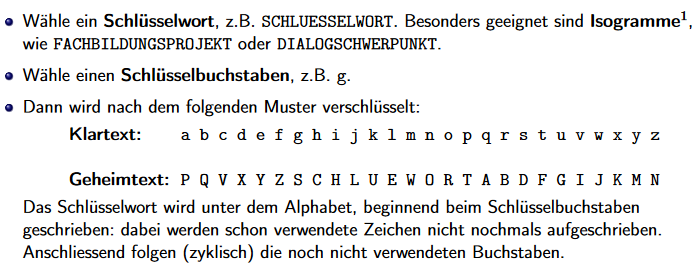
\includegraphics[width=14cm]{img/schluesselwortchiffre.png}

Kann mit Statistik gebrochen werden.\\

\subsection{Vigenère-Chiffre}
Gleich wie Caesar nur mit einem Wort. Also wenn Passwort ``Caesar'' ist,
dann einfach 1. Buchstabe mit 'c' 2. Buchstabe mit 'a' usw. verschieben.\\


\subsection{Asymmetrische Verschlüsselung}
Die drei Phasen des RSA-Algorithmus:
\begin{enumerate}
    \item \textbf{Schlüsselerzeugung:}
    \begin{enumerate}
        \item Zwei Primzahlen $p$ und $q$ wählen und $p \neq q$
        \item Berechne $n = p \cdot q$
        \item Berechne $\phi(n) = (p-1)(q-1)$
        \item Wähle $e$ mit ggT($e, \phi(n)$) = 1
        \item Bestimme $d$, welches ein modulares Inverses zu $e$ modulo $\phi(n)$ ist. Also \\
        $d \cdot e \equiv 1 \mod \phi(n)$
        \item Öffentlicher Schlüssel: $(n, e)$
        \item Privater Schlüssel: $d$
    \end{enumerate}
    \item \textbf{Verschlüsselung:}\\
    $\text{ }\quad c = m^e \mod n$
    \item \textbf{Entschlüsselung:}\\
    $\text{ }\quad m = c^d \mod n$
\end{enumerate}



\newpage
\section{Graphentheorie}
Graphen bestehen aus Knoten und Kanten.\\
Wobei Konten Orte im Netz sind und Kanten Verbindungen zwischen Knoten.\\

Ein ungerichteter Graph $G$ besteht aus einer Knotenmenge $V$ und einer Kantenmenge $E$.\\

wobei jeder Kante $e \in E$ zwei (nicht notwendigerweise verschiedene) Knoten aus $V$ zugeordnet sind.\\

Schreibweise: $e = \{u,v\} = \{v,u\}$\\
Die Knoten $u$ und $v$ heissen dann \textbf{Endknoten} von $e$.\\

Eine Schlinge ist eine Kante, welche einen Knoten mit sich selbst verbindet.\\

Ein Graph, der weder Schlingen noch parallele Kanten enthält, heisst \textbf{einfacher Graph}.\\


\textbf{Beispiel:}\\
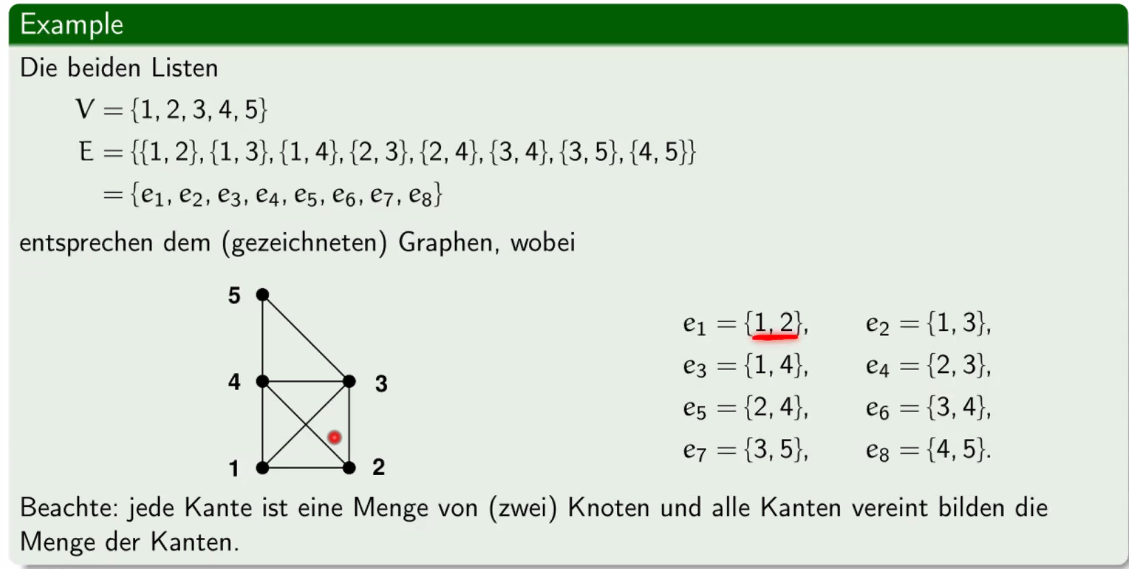
\includegraphics[width=15cm]{img/graphentheorie_beispiel.png}\\



\newpage
\subsection{Knoten- oder Eckengrad}
Der Grad eines Knotens ist die Anzahl der Kanten, die in diesem Knoten enden. Schlingen werden doppelt gezählt\\
Die \textbf{Gesamtsumme} aller Grade ist $2 \cdot |E|$\\

Spezialfälle:\\
$deg(v) = 0 \rightarrow v$ heiss \textbf{isolierte Ecke}\\
$deg(v) = 1 \rightarrow v$ heisst \textbf{Endecke}\\

Eine Gradliste $|V|$ ist eine Liste der Knotengrade eines Graphen.\\

Der \textbf{maximale Grad} eines Graphen wird mit $\Delta (G)$ bezeichnet.\\
Der \textbf{minimale Grad} eines Graphen wird mit $\delta (G)$ bezeichnet.\\



\subsection{Isomorphe Graphen}
\textbf{Definition:}\\
Zwei Graphen $G_1$ und $G_2$ heissen \textbf{isomorph}, wenn es eine Bijektion $f: V_1 \rightarrow V_2$ gibt, so dass für alle $u,v \in V_1$ gilt:\\
$\{u,v\} \in E \Longleftrightarrow \{f(u),f(v)\} \in E'$

Das heisst, dass für jede Kante und jeden Knoten in $G_1$ ein entsprechendes Äquivalent in $G_2$ existiert.\\

Isomorphe Graden haben also gleich viele Knoten und Kanten und deren Gradlisten sind identisch, die Umkehrung gilt jedoch nicht.


\newpage
\subsection{Dijkstra Algorithmus}
\begin{itemize}
    \item $V$ ist die Menge der Knoten
    \item $S$ ist die Menge der Knoten, für welche der kürzeste Weg bereits gefunden wurde
    \item $s$ ist der aktuell gewählte Knoten
    \item $L(v)$ ist die Länge des kürzesten Weges von $s$ nach $v$
    \item $p(v)$ ist der Vorgänger von $v$ auf dem kürzesten Weg von $s$ nach $v$
\end{itemize}
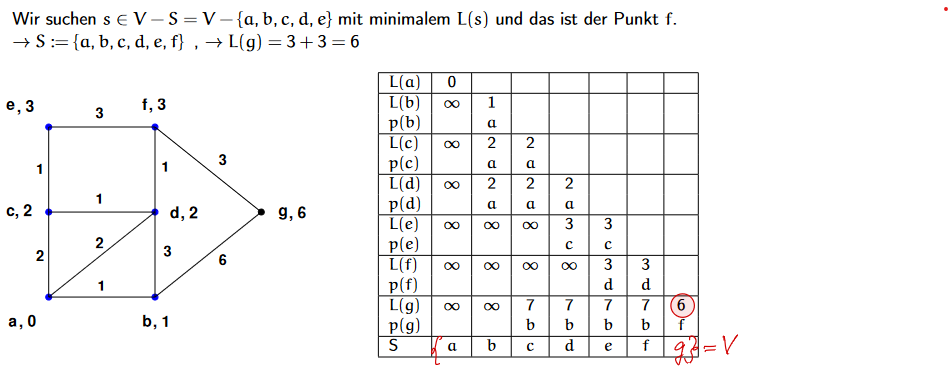
\includegraphics[width=17cm]{img/dijkstra_algorithmus.png}


\newpage
\subsection{Algorithmus von Prim}
Formal:\\

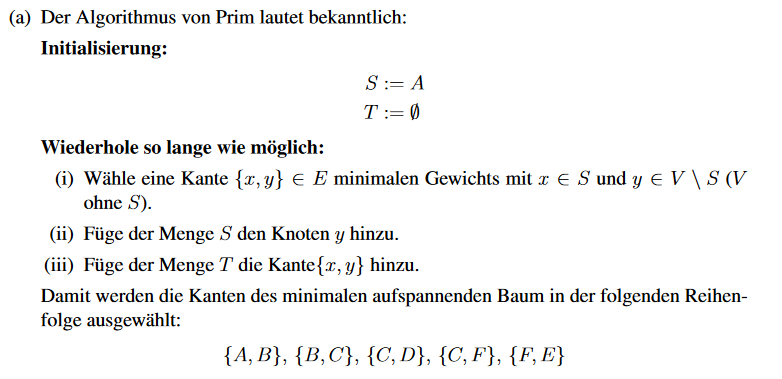
\includegraphics[width=14cm]{img/prim_algorithmus.png}

Einfach:\\
Also immer die Knoten in S anschauen und dann den kürzesten Weg zu einem anderen Knoten in $V$ finden.\\

\newpage
\subsection{Kruskal Algorithmus}
Formal:\\

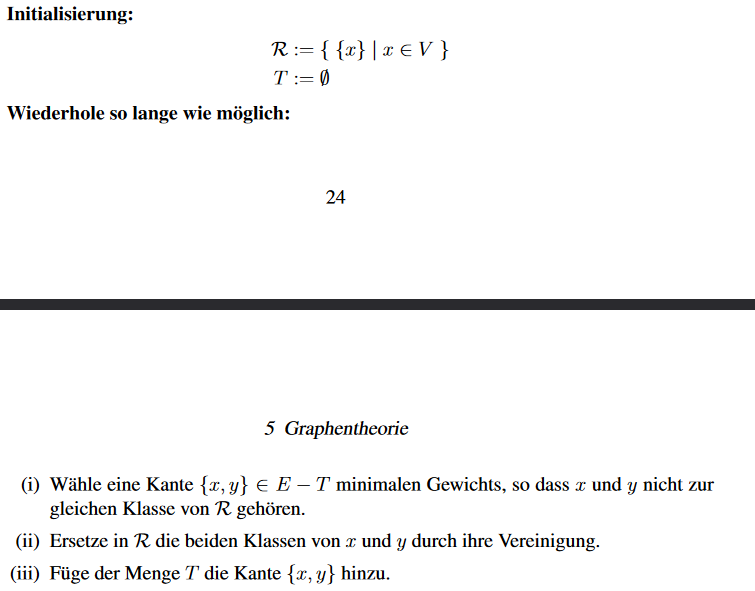
\includegraphics[width=14cm]{img/kruskal_algorithmus.png}\\

Einfach:\\
Immer die kürzeste Kante in allen Bäumen suchen, welche keinen Kreis macht, sie zur Menge 
hinzufügen, bis alle verbunden sind.


\newpage
\subsection{Adjazenzmatrix}
Die Adjazenzmatrix $A(G)$ des Graphen $G$ mit $n$ Knoten ist die $n \times n$ Matrix
mit den Elementen\\
$A_{ij} :=$ Anzahl der Kanten zwischen Knoten $i$ und Knoten $j$.\\

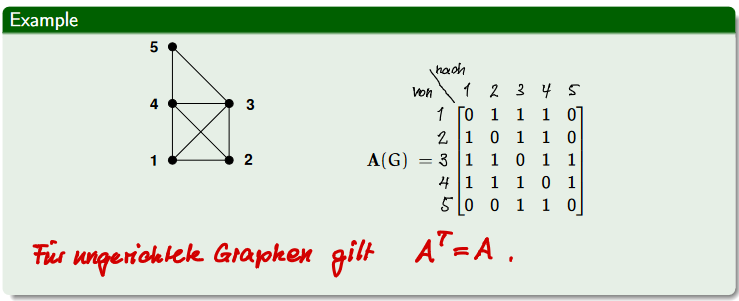
\includegraphics[width=14cm]{img/adjazenzmatrix.png}



\subsection{Inzidenzmatrix}
Die Inzidenzmatrix $B(G)$ ist die $n \times m$ Matrix mit den Komponenten\\
$B_{ij} := \begin{cases}
    1 & \text{falls Knoten $i$ auf Kante $j$ liegt}\\
    0 & \text{sonst}
\end{cases}$\\

Dabei ist $n$ die Anzahl der Knoten und $m$ die Anzahl der Kanten.\\

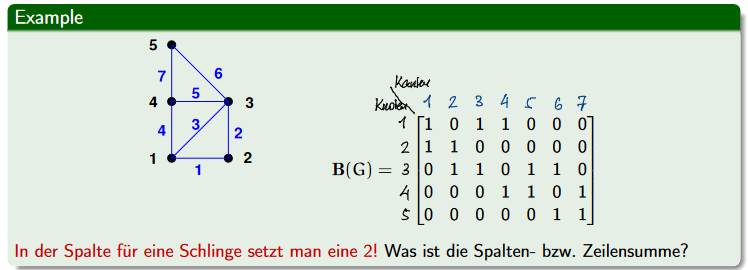
\includegraphics[width=14cm]{img/inzidenzmatrix.png}


\newpage
\subsection{Gradmatrix}
Die Gradmatrix $D(G)$ des Graphen $G$ ist die $n \times n$ Diagonalmatrix, deren 
Diagonaleinträge die Grade der entsprechenden Knoten von $G$ sind.\\

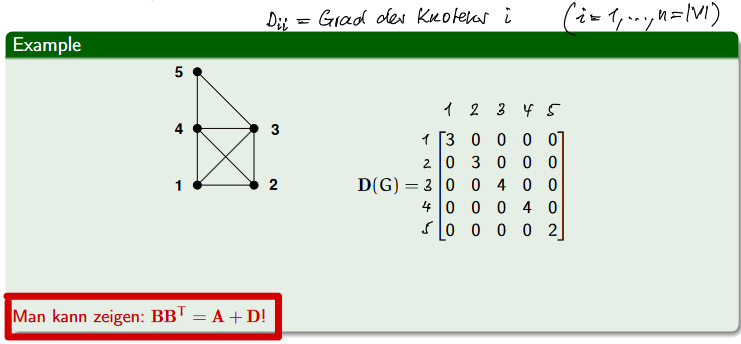
\includegraphics[width=14cm]{img/Gradmatrix.png}

wegen $\mathbf{BB}^T = \mathbf{A + D}$ siehe Admittanzmatrix und Satz von Kirchhoff.

\subsection{Admittanzmatrix}
Admittanzmatrix ist die Differenz aus Gradmatrix $D(G)$ und Adjazenzmatrix $A(G)$ eines Graphen G\\
$L(G) = D(G) - A(G)$



\subsection{Admittanzmatrix - Satz von Kirchhoff}
Es sei $G = (V,E)$ ein Graph und $v \in V$ ein beliebiger Knoten und $L(G)$
die Admittanzmatrix von $G$. Dann ist die Anzahl der Gerüste dieses Graphen durch
$t(G) = det(L_v(G))$ bestimmt (siehe Determinante-Matrizen).\\

\begin{center}
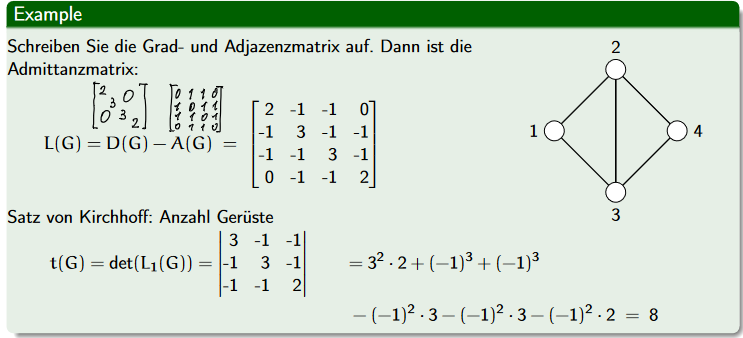
\includegraphics[height=6cm]{img/kirchhoff.png}
\end{center}


\subsection{Planare Graphen}
Ein Graph heisst \textbf{planar}, wenn er sich in der Ebene so zeichnen lässt, dass sich
die Kanten nicht schneiden.\\

Das kann man überprüfen mit dem eulerschen Polyedersatz.\\
Wenn $|V| - |E| + |F| = 2$ ist, dann ist der Graph planar.\\

Wobei
\begin{itemize}
    \item $|V|$ die Anzahl der Knoten ist
    \item $|E|$ die Anzahl der Kanten ist
    \item $|F|$ die Anzahl der Flächen ist
\end{itemize}


\subsection{Färben}
Die kleinste Zahl der Farben wird \textbf{chromatische Zahl} $\chi(G)$ genannt.\\

\subsubsection{Satz von Brooks}
Wenn $G$ ein vollständiger Graph ist giltet.\\
$\chi(K_n) = n$\\
$\delta(K_n) = n - 1$\\

oder ein Kreis:\\
$\chi(C_{2k+1}) = 3$\\
$\chi(C_{2k}) = 2$\\


\newpage
\subsubsection{Chromatische Polynom}
Das chromatische Polynom $P(G,x)$ eines Graphen $G$ ist die Anzahl der Möglichkeiten,
wie $G$ eingefärbt werden kann mit höchstens $x$ Farben.\\

Wenn $G$ ein vollständiger Graph ist gilt:\\
$P(K_n,x) = x(x-1)(x-2) \dots (x-n+1)$\\

Wenn $G$ ein Baum ist, gilt:\\
$P(T_n,x) = x \cdot (x-1)^{n-1}$\\


\subsection{Gerüste / Spannbäume}
Ein Gerüst oder Spannbaum von $G$ ist ein kreisfreier Untergraph (Baum).\\

Ein Baum besitzt genau ein Gerüst.\\

Die Anzahl Gerüste sind $t(G)$.\\



% \begin{align*}
%     587 &= 1 \cdot 392 + 195 \\
% \end{align*}

% Matrix example
% $
% \begin{bmatrix}
%     a_{1,1} & a_{1,2} & a_{1,n}\\
%     a_{2,1} & a_{2,2} & a_{2,n}\\
%     a_{m,1} & a_{m,2} & a_{m,n}
% \end{bmatrix}$\\

% tabular example 3 columns
% \renewcommand{\arraystretch}{1.5}
% \begin{center}
%     \begin{tabular}{ | m{12em} | m{12em} | m{12em} | }
%         \hline
%         1 & 2 & 3\\ 
%         \hline
%         1 & 2 & 3\\ 
%         \hline
%         1 & 2 & 3\\ 
%         \hline
%     \end{tabular}
% \end{center}


% tabular example 2 columns
% \renewcommand{\arraystretch}{1.5}
% \begin{center}
%     \begin{tabular}{ | m{17em} | m{17em} | }
%         \hline
%         1 & 2\\ 
%         \hline
%         1 & 2\\ 
%         \hline
%         1 & 2\\ 
%         \hline
%     \end{tabular}
% \end{center}


% \begin{tikzpicture}[line cap=round,line join=round,>=triangle 45,x=0.5cm,y=0.25cm]
%     \begin{axis}[
%     x=0.75cm,y=0.5cm, % size of the grid
%     axis lines=middle,
%     ymajorgrids=true,
%     xmajorgrids=true,
%     xmin=-10,
%     xmax=10,
%     ymin=-10,
%     ymax=10,
%     xtick={-11,-10,...,10},
%     ytick={-10,-9,...,9},]
%     \draw[line width=2pt,color=blue] (-10,-5) -- (-2,-1);
%     \begin{scriptsize}
%         \draw[color=blue] (-9.866,-4.728) node {$g$};
%         \draw[color=blue] (-1.906,7.172) node {$f$};
%         \draw[color=blue] (3.134,5.232) node {$h$};
%     \end{scriptsize}
% \end{axis}
% \end{tikzpicture}




% \bibliography{quantum_ready}

\end{document}